\documentclass[11pt,prd,letterpaper,amsmath,amssymb,final,nofootinbib
%linenumbers 
,unsortedaddress,superscriptaddress
]{revtex4-1}
% Fun and exciting LaTeX packages!

\pdfoutput=1

%Margins
\usepackage[top=0.9in, bottom=0.9in, left = 0.9in, right=0.9in]{geometry}

\usepackage{graphicx}% Include figure files 
%\usepackage{subfig}
%\usepackage{caption}
%\usepackage{subcaption}
\usepackage{dcolumn}% Align table columns on decimal point
\usepackage{bbm}% blackboard bold
\usepackage{textcomp}% I can't remember what this one does...
\usepackage{color}% Change font colors
\usepackage{gensymb}% Some nice math symbols...
\usepackage{wasysym}
\usepackage{amssymb}
\usepackage{enumerate}
\usepackage{geometry}
\usepackage{setspace}
%\usepackage{hyperref}
%\usepackage{lineno}
\setcounter{tocdepth}{3}

\usepackage[utf8]{inputenc}	%UTF8 file encoding
\usepackage{mathrsfs}
\usepackage{subcaption}
\usepackage[T1]{fontenc}
\usepackage{amssymb,amsmath}
\usepackage{graphicx, amsthm}
\usepackage{booktabs}
  \usepackage{isotope}

  \newcommand{\bvec}[1]{\mathbf{#1}}
  
%\linenumbers
% Begin main document...
\begin{document}

\title{ THEIA: \\ {\small }}

\author{THEIA Collaboration}
\affiliation{Many and Varied}

\maketitle

\section*{Executive Summary}

The  development of new scintillators in combination with high-efficiency, fast photon detection opens up the possibility for discrimination of Cherenkov and scintillation signals in large-scale detectors, offering both high light yield and directional information even at low threshold.  Such a detector, situated in a fully-equipped deep underground laboratory, and utilizing developments in computing and reconstruction techniques, could achieve unprecedented levels of background rejection, thus enabling a physics program that would span topics in nuclear, high-energy, and astrophysics.  

The Theia experiment targets a broad physics program, including a next-generation neutrinoless double beta decay search capable of reaching into the normal hierarchy region of phase space, sensitivity to solar neutrinos, supernova neutrinos, nucleon decay searches, and measurement of the neutrino mass hierarchy and CP violating phase.  

This paper describes the technical breakthroughs that have led to the development of this detector concept, and the potential impact of such a detector on the fields of particle and astrophysics. 

\newpage

\tableofcontents
\setcounter{tocdepth}{5}
\newpage

\section{Introduction and THEIA Overview - GDOG, Bob, JRK, Michi}

The \textsc{Theia}  detector~\cite{asdc} leverages a tried and tested methodology in combination with novel, cutting-edge technology.  
The future of neutrino detection technology lies in massive, high-precision detectors, offering multiple channels for detection.  Current technology is constrained by the choice of target material: water detectors are limited in energy threshold and resolution by the overall light yield of the Cherenkov process, and scintillator detectors are limited in size by optical attenuation in the target itself, and in reconstruction of event direction by the isotropic nature of scintillation light.  

The newly-developed water-based liquid scintillator (WbLS)~\cite{wbls} offers a unique combination of  high light yield and low-threshold detection with attenuation close to that of pure water, particularly at wavelengths $>$ 400~nm.  
Use of this novel target material could allow separation of prompt, directional Cherenkov light from the more abundant, isotropic, delayed scintillation light.  This would be a huge leap forwards in neutrino detection technology, enabling the first low-threshold, directional neutrino detector.  Such a detector could achieve fantastic background rejection using directionality, event topology, and particle ID.  
WbLS chemistry also allows loading of metallic ions as an additional target for
particle detection, including: $^7$Li for charged-current solar neutrino detection; $^{\rm nat}$Gd
for neutron tagging enhancement; 
or isotopes that undergo double beta decay, facilitating a
neutrinoless double-beta decay (NLDBD) program.  The formula and principle of mass-produced WbLS have been developed and demonstrated at the Brookhaven National Laboratory Liquid Scintillator Development Facility.  Metal-doped samples have been produced with high stability, with loadings of up to several percent.  The instrumentation for large-scale liquid production is currently under design.

\textsc{Theia} would combine the use of a 30--100-kton WbLS target, doping with a number of potential isotopes, high efficiency and ultra-fast
timing photosensors, and a deep underground location.  A potential site is the Long Baseline Neutrino Facility (LBNF) far site, where \textsc{Theia} could operate in conjunction with the liquid argon tracking detector proposed by DUNE~\cite{dune}.  
The basic elements of this detector are being developed now in experiments such as WATCHMAN~\cite{wm}, ANNIE~\cite{annie} and SNO+~\cite{snopl}.  

A large-scale WbLS detector such as \textsc{Theia} can achieve an impressively broad program of physics topics, with enhanced sensitivity beyond that of previous detectors.  Much of the program hinges on the capability to separate prompt Cherenkov light from delayed scintillation.  This separation provides many key benefits, including:
\begin{itemize}
\item The ring-imaging capability of a pure water Cherenkov detector (WCD).  This enables a long-baseline program in a scintillation-based detector, with the additional benefit of low-threshold detection of hadronic events.

\item  Direction reconstruction using prompt Cherenkov photons.   This allows statistical identification of events such as solar neutrinos, which offer a rich physics program in their own right, as well as forming a background to many rare-event searches, including NLDBD and nucleon decay.

\item Low thresholds and good energy and vertex resolution using the abundant scintillation light.

\item Detection of sub-Cherenkov threshold scintillation light.  This provides excellent particle identification, including enhanced neutron tagging, detection of sub-Cherenkov threshold particles such as kaons in nucleon decay searches, and separation of atmospheric neutrino-induced neutral current backgrounds for inverse beta decay searches.

\end{itemize}

One of the most powerful aspects of \textsc{Theia} is the flexibility:  in the target medium itself, and even in the detector configuration.  The WbLS target can be tuned to meet the most critical physics goals at the time by modifying features of the target cocktail, including: the fraction of water vs scintillator; the choice of wavelength shifters and secondary fluors; and the choice of loaded isotope.  There is also the potential to construct a bag to contain isotope, and perhaps a higher scintillator-fraction target, in the centre of the detector, building on work by KamLAND-Zen~\cite{klz} and Borexino~\cite{bor}.  


\subsection{Detector configuration}
Include TWO baseline designs -- ideal and ``realistic'' (existing cavern)

Include description of phased deployment
e.g. refer to THEIA-i, THEIA-ii, THEIA-iii

Define the baseline design for each here, so that physics sections can simply refer back

e.g. THEIA-ii might be 50ktonne 10\% WbLS, 90\% coverage

whereas THEIA-iii might be the above with 5\% WbLS but a bag containing LS + Te/Xe


\section{Technology Developments}
\subsection{Water-based Liquid Scintillator - R. Svoboda}

\subsection{Photon Sensors - \bf volunteers?}
\subsection{Reconstruction Techniques -- B. Wonsak \& M. Tsanov}
%Including techniques and results (to date) for both low and high energy events

%\documentclass[a4paper]{article}
%
%%% Language and font encodings
%\usepackage[english]{babel}
%\usepackage[utf8x]{inputenc}
%\usepackage[T1]{fontenc}
%\usepackage[noadjust]{cite}
%\usepackage{booktabs}
%\usepackage{subcaption}
%\renewcommand{\citedash}{--}  
%%% Sets page size and margins
%\usepackage[a4paper,top=3cm,bottom=2cm,left=3cm,right=3cm,marginparwidth=1.75cm]{geometry}
%
%%% Useful packages
%\usepackage{amsmath}
%\usepackage{url}
%\usepackage{graphicx}
%%\usepackage[colorinlistoftodos]{todonotes}
%\usepackage[colorlinks=true, allcolors=blue]{hyperref}
%
%\title{\textsc{Theia} DBD White Paper}
%%\author{T. Klosterman, V. Lozza, A. Mastbaum}
%
%\begin{document}
%\maketitle

%\section{Introduction}
The \textsc{Theia} search for neutrinoless double beta decay (NLDBD) aims for
sensitivity to the non-degenerate normal hierarchy parameter space
within the canonical framework of light Majorana neutrino exchange and
three-neutrino mixing, at the level of $m_{\beta\beta}\sim5$ meV.
This is achieved through the loading of a very large
mass of a NLDBD candidate isotope into an ultra-pure liquid scintillator
target, together with coincidence and topological particle identification
techniques.

\subsubsection{Detector Configuration}
\paragraph{Target Medium}
For the present studies, we consider a target that consists of pure LAB
liquid scintillator loaded with the NLDBD isotope. This volume is contained
within a nylon balloon, and the region of the detector outside is
filled with water-based liquid scintillator (WbLS) with no isotope loading.
With loading at 3\% by mass, a 25 ton (50 ton) experiment corresponds to a
6.4 m (8 m) radius containment balloon.

The mass of LAB is obtained using a density of 0.86 g/cm$^3$, the optics are
based on measurements by the SNO+ collaboration, and the backgrounds are based
on measurements by SNO+, Borexino, and KamLAND-Zen.

\paragraph{Isotope Loading}
We consider possible NLDBD searches using two candidate isotopes: Te and Xe.
In the case of Xe loading, xenon gas 89.5\% enriched in $^{136}$Xe is
dissolved directly into
the liquid scintillator, while Te loading is achieved via a novel
technique developed for the SNO+ experiment
and uses natural Te (34.1\% $^\mathrm{130}$Te).
The contamination associated with the materials used for Te loading are
considered in the background assessment.

Additional NLDBD isotopes may be considered as long as they can be loaded into
liquid scintillator. A staged approach is envisioned where an
NLDBD observation in one isotope can be confirmed by removing it and deploying
a second; the ability to switch isotopes is a key advantage of a liquid
scintillator detector.

\subsubsection{Backgrounds}
The main sources of background near the NLDBD energy region of interest
include:
\begin{description}
\item[Double Beta Decay] This irreducible background is due to the
$2\nu\beta\beta$ decays of $^{130}$Te or $^{136}$Xe. Due to the steeply-falling
spectrum, the number of events falling in the ROI depends strongly on the
energy resolution.
\item[Cosmogenic Production] These backgrounds are due to activation of nuclei
by muons (during data taking) or protons and neutrons (during material
production and handling at Earth's surface).
\item[Solar Neutrinos] The primary source is elastic scattering of $^{8}$B
solar neutrinos, though these events can potentially be reduced using the
direction relative to the Sun. Another potential background is due to
activation of the target material (Te or Xe) by the solar neutrinos,
mainly $^{7}$Be and $^{8}$B neutrinos; this background is also dependent
on the energy resolution.
\item[Internal Contamination] Decays from U- and Th-chain impurities
present in the scintillator mixture. Due to the large $Q$ value of the
candidate NLDBD isotopes, the two important backgrounds are due to
$^{214}$Bi ($Q=3.27$ MeV) and $^{208}$Tl ($Q=5$ MeV). The scintillator
purity can be improved by purification techniques to levels better than
$10^{-18}$, as demonstrated by the Borexino experiment \cite{bxo16}.
\item[External Sources] Decays from U and Th-chain impurities present
in the balloon material, the external water-based liquid scintillator, the
shielding water, and in the PMTs also contribute to the background. The
two most important isotopes are $^{214}$Bi and $^{208}$Tl, as they decay by
the emission of high energy ($E>2$ MeV) $\gamma$ rays that can travel long
distances. These events can be reduced using a fiducial volume cut, though the
balloon material remains the most important as it is closest to the target
volume.
\end{description}
A summary of all the expected background events is given in Table
\ref{tab::bckg}.

\begin{table}[t]
\centering
\begin{tabular}{lccc}
\toprule
                                            &                                              & \multicolumn{2}{c}{\bf Expected events/y}     \\
{\bf Source}                                & {\bf Target level}                           & $r = 6.4$ m           & $r = 8$ m             \\
\midrule
Balloon $^{10}$C                            &                                              & 250 -- 800            & 500 -- 1600           \\
$^{8}$B neutrinos                           &                                              & 1490                  & 2950                  \\
$^{130}$I (Te target)                       &                                              & 48 (9 from $^{8}$B)   & 93  (18 from $^{8}$B) \\
$^{136}$Cs (Xe target)                      &                                              & 24 (3 from $^{8}$B)   & 47 (6 from $^{8}$B)   \\
$^{136}$Cs ($^\mathrm{enr}$Xe target)       &                                              & 245 (35 from $^{8}$B) & 478 (68 from $^{8}$B) \\
2$\nu\beta\beta$ (Te target)                &                                              & 3.8$\times$10$^{7}$   & 7.4$\times$10$^{7}$   \\  
2$\nu\beta\beta$ (Xe target)                &                                              & 3.6$\times$10$^{6}$   & 7.0$\times$10$^{6}$   \\  
2$\nu\beta\beta$ ($^\mathrm{enr}$Xe target) &                                              & 3.6$\times$10$^{7}$   &  7.1$\times$10$^{7}$  \\  
Liquid scintillator                         & $^{214}$Bi: $10^{-17}$ g$_{U}$/g             & 3700                  & 7300                  \\
                                            & $^{208}$Tl: $10^{-17}$ g$_{Th}$/g            & 440                   & 870                   \\
Nylon Vessel                                & $^{214}$Bi: 1.1$<\times10^{-12}$ g$_{U}$/g   & 7.7$\times$10$^{4}$   & 1.2$\times$10$^{5}$   \\
                                            & $^{208}$Tl: 1.6$<\times10^{-12}$ g$_{Th}$/g  & 1.3$\times$10$^{4}$   & 2.1$\times$10$^{4}$   \\
PMTs                                        & $^{214}$Bi: $10^{-6}$ g$_{U}/$PMT            &                                               \\
                                            & $^{208}$Tl: $10^{-6}$ g$_{Th}/$PMT           &                                               \\
\bottomrule
\end{tabular}
\caption{Dominant background sources expected for the NLDBD search in
\textsc{Theia}. It is assumed that the Te or Xe isotopes are directly
loaded at a level of 3\% in the LAB+PPO scintillator cocktail, for a
total mass of 28.3 tonnes (6\,m radius) or 55\,tonnes (8\,m radius).}
\label{tab::bckg}
\end{table}

\paragraph{Cosmogenic Backgrounds}
The cosmogenically-induced background consists of nuclides produced by
activation of the target material by neutrons, protons, and muons during
production, handling, storage, and data-taking.

Long-lived, high $Q$ value nuclides can be produced by neutron and proton
activation mainly while the material is on the Earth's surface. The production
in Xe and Te has been investigated by several authors
\cite{mei09, baudis15, zhang16, norm05, bard97, wang15, lozza15}. Among
the most important nuclides are $^{60}$Co ($Q=2.8$ MeV, $T_{1/2}=5.27$ y) and
$^{110m}$Ag ($Q=3.1$ MeV, $T_{1/2}=250$ d). Mitigation of these background
sources requires minimal exposure at sea level, a deep underground cool-down
period, and chemical purification processes \cite{snop16}.

Neutron activation can also happen deep underground, while the experiment is
running. Neutrons originate from the radioactivity and from muon-induced
reactions in the rock. A water shield will provide a mitigation, as the
majority of the neutrons will thermalize and stop before reaching the target
material.

For the purpose of this paper, it is assumed that the material will have a
minimum exposure time at sea level and will be stored underground long
enough to allow all the potential cosmogenic-induced nuclides produced during
the surface exposure to decay.\\

A different source of cosmogenic background is the muon activation of the
material during the data-taking period. In particular a potential background
is the production of $^{10}$C ($Q=3.65$ MeV, $T_{1/2}=19.3$ s) by muon
interaction with the carbon atoms of the liquid scintillator. The interaction
is accompanied by the emission of two neutrons. $^{10}$C decays via the
emission of a positron of 1.87\,MeV end-point energy, followed by the
emission of a $\gamma$ of 0.72\,MeV total energy. A mitigation strategy for
this background source consists of a three-fold coincidence technique as
developed by Borexino and KamLAND \cite{galb05, gando16}, making use of the
muon trajectory, the 2.2\,MeV $\gamma$ emitted by the neutron capture, and
the $^{10}$C decay. Additionally, the $\gamma$ may travel away from the
positron stopping point several tens of centimeters. This event topology is
different from the neutrinoless double-beta decay, in which the energy
deposition is localized.

The event rate of muon induced $^{10}$C decays can be estimated following
Reference \cite{hagn00}. The muon flux expected at the Homestake 4850 level
(4300 mwe) is $4.2\times10^{-9}$ cm$^{-2}$ s$^{-1}$, while the calculated
average muon energy at the same depth is 293\,GeV \cite{mei06}. The
LAB+PPO mixture has a $^{12}$C density of $4.4\times 10^{31}$ atoms/kt.
The following formula can be used to scale the density from the one measured
in Borexino and KamLAND:
\begin{equation}
R_{i} = R_{data} \times 
{\left( \frac{\langle E_{\mu} \rangle}
             {\langle E_{\mu, data} \rangle} \right) }^{\alpha_{sim}} \times
\frac{\Phi_{\mu}}{\Phi_{\mu, data}} \times
\frac{n_{12C}}{n_{12C, data}}
\end{equation}
where $\alpha_{sim}$ has been obtained from FLUKA/Geant4 simulation and is
equal to 0.7621 for $^{10}$C \cite{zbiri10}. This results in about 300
events/kt/yr. Using Equation 10 in Reference \cite{hagn00} results in about
800 events/kt/yr. For this source of background a reduction of 92.5\% is assumed based on what reached by Borexino \cite{bxo2013}

\paragraph{Solar Neutrino Induced Background}
$^{8}$B solar neutrino elastic scattering in the target material results in
a background that is approximately flat across the NLDBD energy region of
interest. The spectrum can be normalized using the total $^{8}$B flux and
best fit solar mixing parameters, as in Reference \cite{SNO_3ph}. The expected
rate is about 1200 events/yr/kt of target material.\\

Another source of background are the nuclides produced by charged current
interaction of solar neutrinos with Te or Xe, in particular $^{130}$Te and
$^{136}$Xe. A detailed study of the expected interaction rate is given in
References \cite{eijiri14, eijiri17}. 

For $^{130}$Te (34.08\% natural abundance) a total of 33.7 SNU are expected,
of which 6.1 SNU due to $^{8}$B neutrinos and 20.9 SNU due to $^{7}$Be
neutrinos. The daughter isotope is $^{130}$I in the 1$^{+}$ excited state.
The excited states decay quickly to the first excited level, which decays with
$T_{1/2}=8.84$ min to the ground state via internal transition (branching
ratio 84\%, $E_\gamma=40$ keV), or directly beta decays to $^{130}$Xe with a
$Q$ value of 2.99\,MeV (BR = 16\%). The ground state beta decays with a
$Q$ calue of 2.95\,MeV and a $T_{1/2}=12.4$\,h. Due to the long half life a
tagging technique based on a delayed coincidence might have a small efficiency.

For $^{136}$Xe (8.8573\% natural abundance) a total of 68.8 SNU are expected,
of which 9.8 SNU due to $^{8}$B neutrinos and 46 SNU due to $^{7}$Be neutrinos.
The resulting isotope is $^{136}$Cs in the 1$^{+}$ excited states. The
excited states decay quickly to the ground state, which decays with
$T_{1/2}=13.16$\,d via beta decay (branching ratio = 100\%) with a $Q$ value
of 2.55\,MeV. Again in this case, a tagging technique
based on a delayed coincidence will have only a small effect on removing this
source of background due to the long half life.

The expected rate of events is given in Table \ref{tab::bckg}.

\paragraph{Double Beta Decay Backgrounds}

The number of 2$\nu\beta\beta$ decays for $^{130}$Te is calculated using the
half life measured by CUORE \cite{Cuore017},
$T_{1/2}=(8.2\pm0.2~\mathrm{(stat.)}\pm0.6~\mathrm{(syst.)})\times 10^{20}$ y.
This results in a rate of events per year
\begin{equation}
R_{2\nu\beta\beta} = 1.33 \times 10^{7} \times M \times f
\end{equation} 
where $M$ is the mass inside the balloon in kt and $f$ is the loading fraction
of natural isotope, or $3.8\times10^7$ events/yr for the 3\% loading and a
6.4\,m radius balloon.\\
 
For $^{136}$Xe, the half life measurement in \cite{gando16, exo14} is used,
$T_{1/2}=(2.165\pm0.016~\mathrm{(stat.)}\pm0.059~\mathrm{(syst.)})\times10^{21}$
y, for a rate of
\begin{equation}
R_{2\nu\beta\beta} = 1.26 \times 10^{6} \times M \times f
\end{equation} 
or $3.6\times10^6$ events/y for the 3\% loading and a 6.4\,m radius balloon.
In case a 89.5\% enriched $^{136}$Xe is used, the expected number of events is
3.6$\times$10$^{7}$ events/yr within a 6.4\,m radius balloon.
 
\paragraph{Scintillator Backgrounds}
A high purity level required in the LAB+PPO cocktail used to fill the balloon
can be obtained using various purification techniques, including liquid-liquid
extraction, nano-filtration, steam stripping, and distillation. A level
of 10$^{-17}$ g/g in both U and Th has been demonstrated by the
KamLAND \cite{kam03} and the Borexino \cite{bxo09} experiments. More recently
a purity level of better than 10$^{-18}$ has been obtained for the Phase-II
of Borexino \cite{bxo16}:
\begin{description}
\item[$^{238}$U] $<$ 9.7 $\times$ 10$^{-19}$ g/g (95\% CL from $^{214}$Bi-Po)
\item[$^{232}$Th] $<$ 1.2 $\times$ 10$^{-18}$ g/g (95\% CL from $^{212}$Bi-Po)
\end{description}

In addition to chemical purification, delayed coincidence techniques can
be used to reduce the number of $^{214}$Bi decays falling in the ROI.
$^{214}$Bi ($T_{1/2}$ = 19.9\,min) beta decays to $^{214}$Po with a $Q$ value
of 3.27\,MeV in 99.979\% of cases. Several experiments have shown that this
decay can be tagged using the subsequent $^{214}$Po alpha-decay
($T_{1/2}$ = 164.3\,$\mu$s, E$_{\alpha}$ = 7.7\,MeV). A rejection of
approximately 100\% for $^{214}$Bi decays falling the ROI has been shown as
possible by the SNO+ experiment.
In the remaining 0.021\% of the cases $^{214}$Bi alpha-decays to $^{210}$Tl
($T_{1/2}$ = 1.3\,min), which beta decays to $^{210}$Pb with a $Q$ value of
5.5\,MeV. An $\alpha$--$\beta$ delayed coincidence, can be applied in this
case. However, due to the longer half-life of $^{210}$Tl, the tagging
technique is expected to be less efficient.

In the case of the Th chain, the most relevant isotope is $^{208}$Tl
($T_{1/2}$ = 3.0\,min, 36\% branching ratio), which beta decays to $^{208}$Pb
with a $Q$ value of 5.0\,MeV. An $\alpha$--$\beta$ delayed coincidence can
help in the reduction of the number of isotopes falling in the ROI. However,
also in this case, the longer half life will result in a smaller rejection
factor compared to the $^{214}$Bi case.\\

In addition to the LAB+PPO cocktail purity, any material associated with the
NLDBD loading must be considered. SNO+ reports a target level after the
0.5\% Te loading of around 10$^{-15}$ and
10$^{-16}$ g/g for the U-238 and the Th-232 chains, respectively.
KamLAND-Zen \cite{gando13} reports a purity of 
(1.3 $\pm$ 0.2) $\times$ 10$^{-16}$ g/g U and
(1.8 $\pm$ 0.1) $\times$ 10$^{-15}$ g/g Th.
Higher purity levels are achievable in principle by improving the target
material purification technique, like the purity of the chemicals used to process the tellurium. A target purity of 10$^{-17}$ g/g for both the U and Th chain has been
assumed for the \textsc{Theia} experiment. This purity level require a reduction factor of 99.9\% of the $^{214}$Bi events in the ROI in order to reduce the internal background to a negligible level. Factor 10 worse purity would require a factor 10 better background reduction. The SNO+ experiment has shown that it is possible to reach a reduction of the $^{214}$Bi background of more than 99.99\% in the region of interest.%

\paragraph{Balloon Backgrounds}
Among the external background sources, the closest to the target volume are
the $^{214}$Bi and $^{208}$Tl decays in the containment balloon. A typical
balloon material is nylon, and the intrinsic purity levels can be found in
\cite{radiopurityorg}. The values, based on Borexino measurements, are
1.1 ppt and 1.6 ppt for U and Th, respectively. KamLAND-Zen has also measured
the purity level of the nylon they used for their balloon. Results
in Reference \cite{kamLAND_Zen} give 2 ppt and 3 ppt for U and Th, respectively.
The purity levels reached by Borexino are used as target levels for the
\textsc{Theia} experiment. A nylon balloon with a thickness of about 45$\mu$m is assumed.

\paragraph{PMT Backgrounds}
For the present discussion it is assumed that with a fiducial volume cut the
background induced by the PMTs is negligible in the region of interest for
\textsc{Theia} NLDBD studies.

\subsubsection{NLDBD Sensitivity}
\label{sec::sensitivity}
\paragraph{Detector Modeling}
In order to study sensitivity to NLDBD in \textsc{Theia}, the dominant
backgrounds have been simulated using the Geant4-based RAT-PAC software
package.\footnote{\url{https://github.com/rat-pac/rat-pac}}
The detector is modeled as a cylinder with 40\,m radius and height, for a
total mass of 50\,kt, located in the Homestake mine at a depth of 4300\,m.w.e.
A PMT coverage of 5\% has been used for the simulations, then rescaled
according to the assumed light yield.

The model assumes a liquid scintillator contained in the balloon
composed of LAB with 2\,g/l PPO, while the volume outside the balloon is
filled with a WbLS (10\% LAB-PPO and 90\% water). The optical properties of
the LAB-PPO cocktail have been measured by the SNO+ collaboration. For the
WbLS, the optical properties are obtained by weighting contributions of the
LAB-PPO and water, and are consistent with benchtop measurements.
A multi-component absorption and reemission model (i.e. separate absorption
lengths and reemission probabilities for each of the cocktail component) are
used in the simulation. Radioactive decays are simulated using the Decay0
code \cite{decay0}.

While event reconstruction algorithms remain under development, the
reconstructed energy is approximated by assuming the Poisson limit of
photon counting: the true deposited energy, accounting for quenching, is
smeared out by a Gaussian resolution function corresponding to the light
yield. As a baseline, an average light yield of 1200 PMT hits per deposited
MeV is assumed (corresponding to about 3\%/$\sqrt(E)$ energy resolution), except where noted.

\paragraph{Counting Analysis}
To estimate the sensitivity, a single-bin counting analysis is employed. Since
all backgrounds do not scale with isotope mass (e.g. solar neutrinos
and external $\gamma$ backgrounds), we use the Monte Carlo to evaluate the
background expectation, establish a confidence region using the Feldman-Cousins
frequentist approach, and derive an expected limit on the NLDBD half life:
\begin{equation}
\label{eq:sens}
\widehat{T}_{1/2}^{0\nu\beta\beta}(\alpha) = 
\frac{N\cdot \epsilon \cdot t \cdot \ln 2}{\mathrm{FC}(n=b, b; \alpha)}
%\widehat{T}_{1/2}^{0\nu\beta\beta}(\alpha) = \left\langle
%\frac{n\cdot \epsilon \cdot t \cdot \ln 2}{\mathrm{FC}(N, b; \alpha)}
%\right\rangle_{n=\mathrm{Pois}(b)}
\end{equation}
where $N$ is the number of atoms of active NLDBD isotope, $\epsilon$ is the
efficiency, $t$ the live time, and $b$ the expected background.
`FC' refers to a Feldman-Cousins interval at confidence level
$\alpha$.

The NLDBD region of interest is defined by a a fiducial volume cut and
energy window. The fiducial volume is 7 m for an 8 m radius balloon, which
reduces backgrounds from the balloon material. The energy window is asymmetric
about the $Q$ value, from $-\sigma/2 \to 2\sigma$ of a Gaussian fit to the
NLDBD signal peak; this maximizes signal acceptance ($\epsilon=66.9$\%)
while removing much of the steeply-falling two-neutrino DBD background
spectrum.

To summarize the baseline background assumptions detailed above,
we use a reduction
factor for $^{10}$C of 92.5\%, $^{214}$Bi 99.9\%, balloon backgrounds 50\%,
and $^8$B solar neutrinos 50\%.

The expected event rates per year for a $^\mathrm{nat}$Te or
$^\mathrm{enr}$Xe loaded \textsc{Theia}
detector with an 8 m radius containment balloon are given in Table
\ref{tab:counts}. In both cases, the loading is at the level of 3\% by mass.
In the Xe case, enrichment to 89.5\% $^{136}$Xe is used, while Te is in its
natural form (34.1\% $^{130}$Te). Figure \ref{fig:spectrum-plots} shows
the background spectra near the endpoint in the
Te (Figure \ref{fig:spectrum-te}) and Xe (Figure \ref{fig:spectrum-xe}) cases.

\begin{table}
\centering
\begin{tabular}{ccc}
\toprule
                          & \multicolumn{2}{c}{\bf Events/ROI$\cdot$y} \\
{\bf Signal}              & Te Loading & $^{enr}$Xe Loading \\
\midrule
$0\nu\beta\beta$ (10 meV) & 65.4       & 116.4      \\
\midrule
$2\nu\beta\beta$          & 48.0       & 38.2       \\
$^8$B Solar ES  (50\%)           & 138.5      & 138.4      \\
$^{10}$C  (92.5\%)                & 24.6       & 25.4       \\
$^{130}$I                 & 48.3       & ---        \\
$^{130m}$I                & 1.7        & ---        \\
$^{136}$Cs                & ---        & 0.57       \\
$^{208}$Tl                & 0.02       & 0.002      \\
$^{214}$Bi  (99.9\%)               & 4.0        & 4.4        \\
Balloon $^{214}$Bi  (50\%)       & 24.0       & 27.4       \\
Balloon $^{208}$Tl  (50\%)      & 0.25       & 0.14       \\
\midrule
{\bf Total}               & 289.5      & 234.5      \\
\bottomrule
\end{tabular}
\caption{Expected background counts per year in the ROI. In parenthesis is shown the reduction factor applied.}
\label{tab:counts}
\end{table}

\begin{figure}
\centering
\begin{subfigure}[b]{0.49\textwidth}
 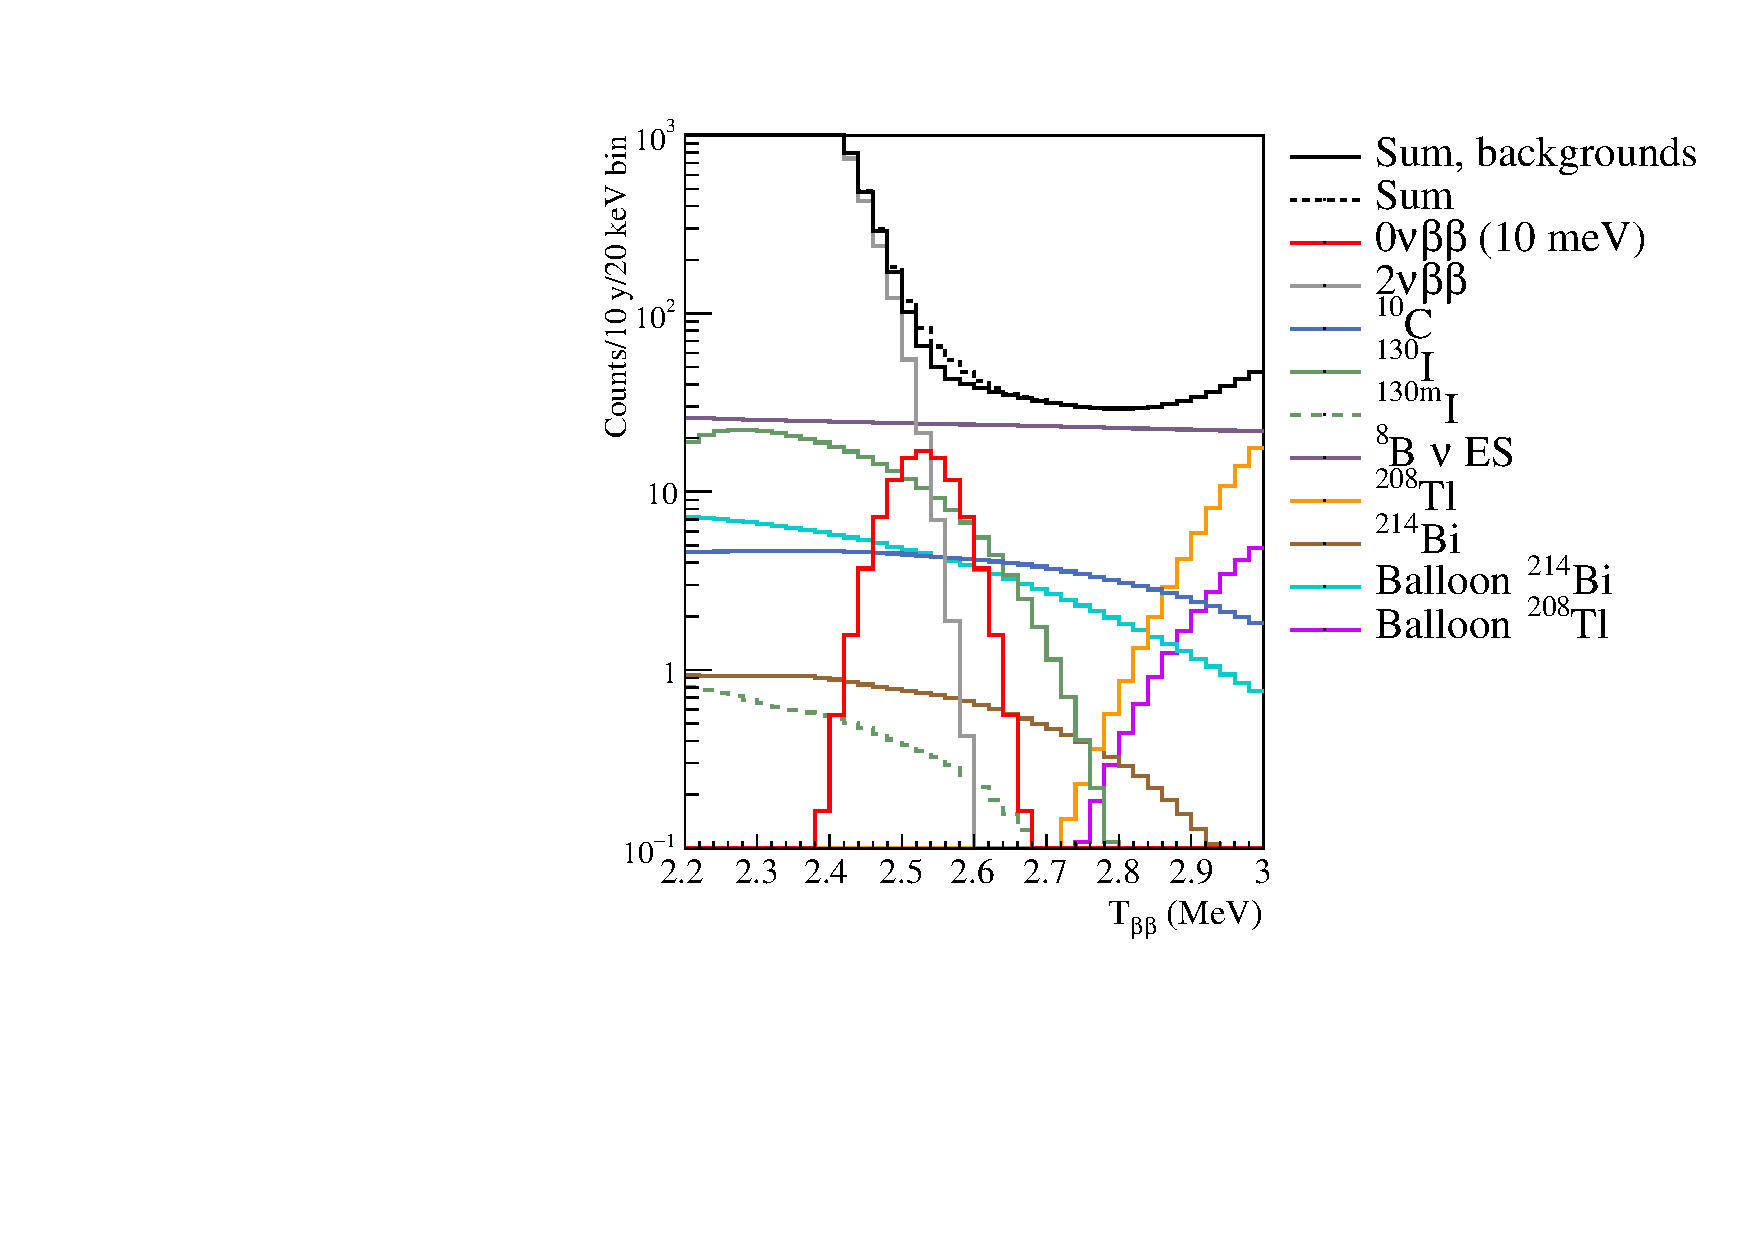
\includegraphics[width=\textwidth]{dbd/spectrum_plot_te.pdf}
 \caption{Te loading}
 \label{fig:spectrum-te}
\end{subfigure}
\begin{subfigure}[b]{0.49\textwidth}
 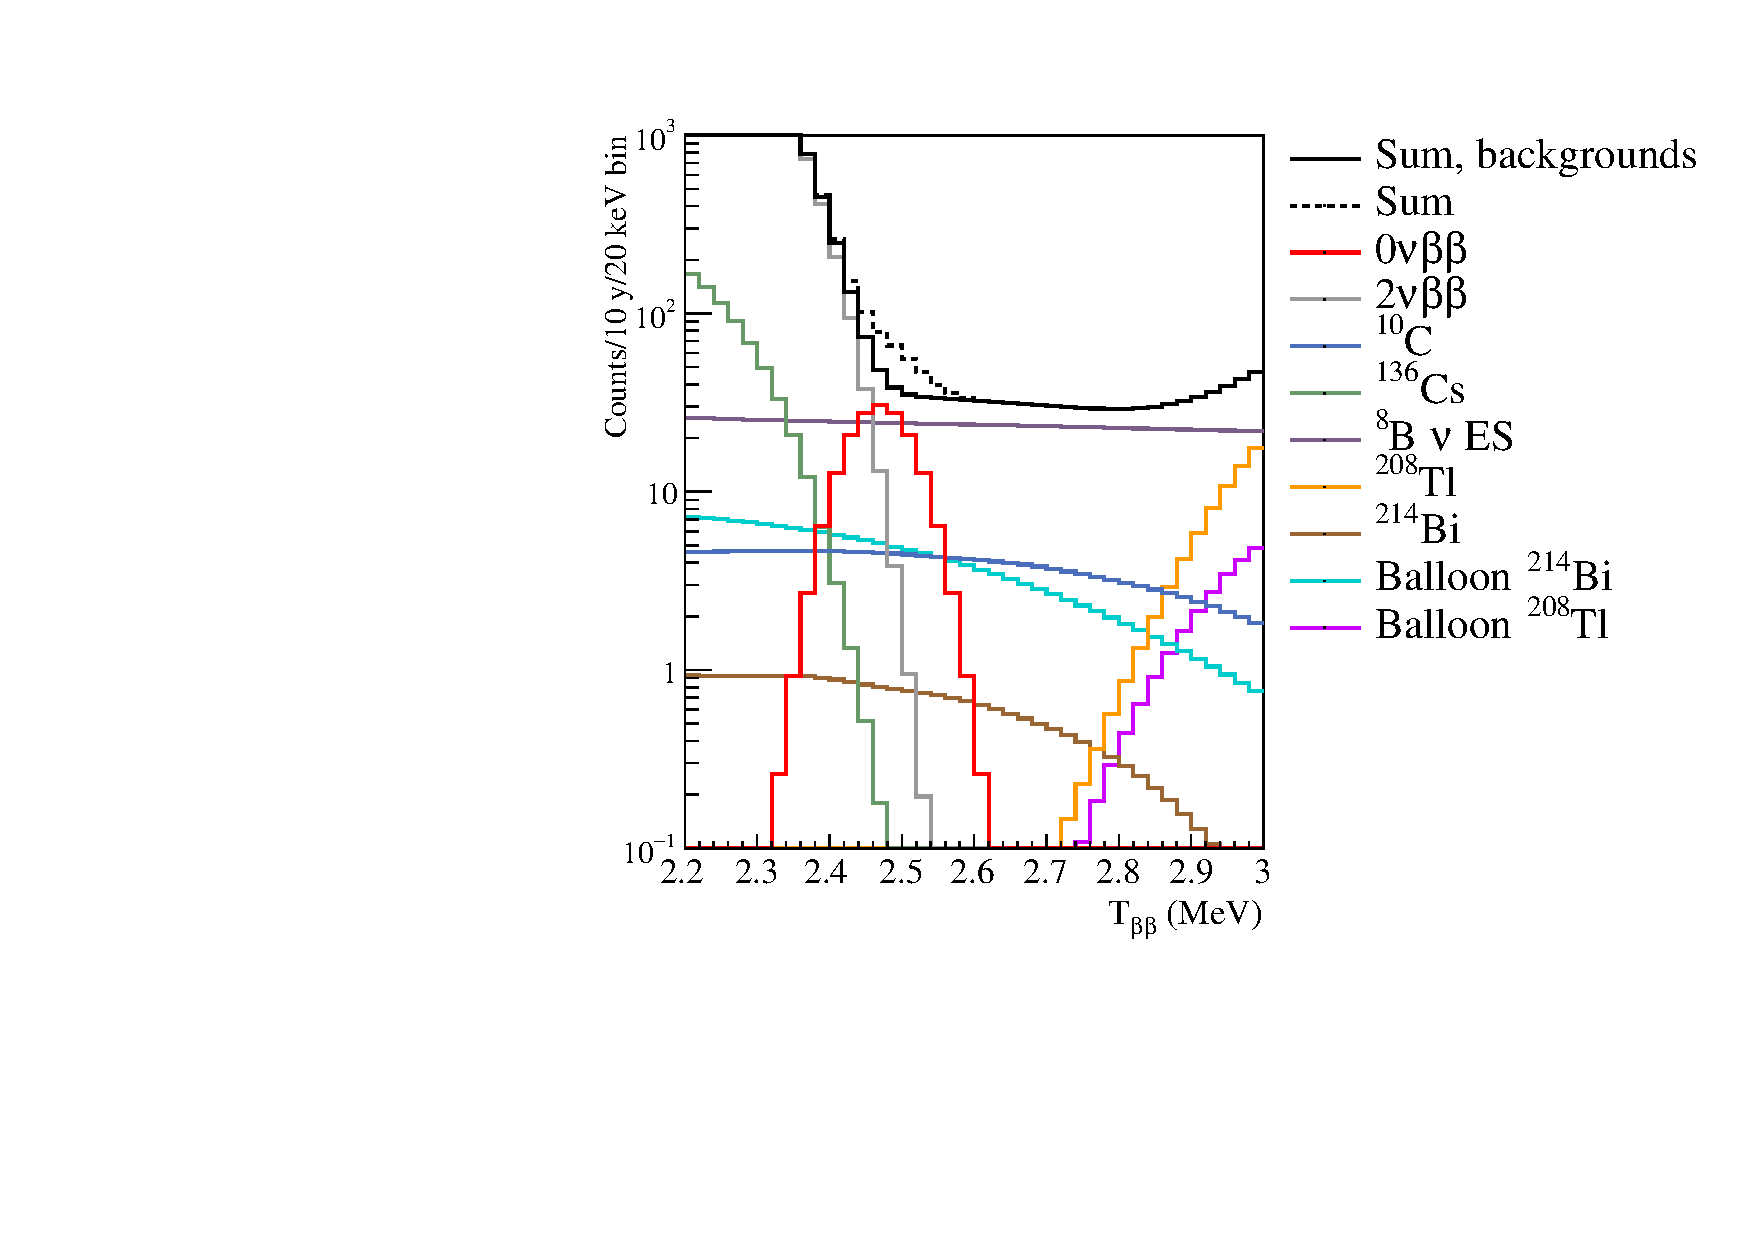
\includegraphics[width=\textwidth]{dbd/spectrum_plot_xe.pdf}
 \caption{Xe loading}
 \label{fig:spectrum-xe}
\end{subfigure}
\caption{Energy spectra near the NLDBD endpoint for events within the 7 m
fiducial volume.}
\label{fig:spectrum-plots}
\end{figure}

Following Equation \ref{eq:sens}, we obtain a sensitivity in terms of
$\hat{T}_{1/2}^{0\nu\beta\beta}$, and compute a corresponding limit on
the effective Majorana neutrino mass $m_{\beta\beta}$ assuming a light
neutrino exchange model with phase space factors from
Kotila and Iachello \cite{2012PhRvC..85c4316K} and using the IBM-2 matrix
element \cite{Barea:2013wb} for definiteness. The 90\% CL sensitivity
is:
\[
\mathrm{\bf Te:}~~
  T_{1/2}^{0\nu\beta\beta} > 9.7\times10^{27}~\mathrm{y},~
  m_{\beta\beta} < 6.7~\mathrm{meV}
\]
\[
\mathrm{\bf Xe:}~~
  T_{1/2}^{0\nu\beta\beta} > 2.6\times10^{28}~\mathrm{y},~
  m_{\beta\beta} < 4.9~\mathrm{meV}
\]

\noindent
%{\bf TODO:} Comment on prohibitive Xe costs?

\subparagraph{Energy Resolution}
The sensitivity is strongly dependent on the energy resolution, which in turn
depends on the total detected light yield, since this sets of the level to
which events in the steeply-falling $2\nu\beta\beta$ decay spectrum can
migrate into the NLDBD energy ROI. Figure \ref{fig:scale-ly} shows the
impact, holding other assumptions fixed.

\subparagraph{Solar Neutrinos}
It is possible in principle to discriminate solar neutrino interactions from
NLDBD signal, using Cherenkov light to determine the direction with respect
to the Sun and possibly separate one- and two-ring topologies, on a
statistical basis if not event-by-event. This is particularly important for
\textsc{Theia}, where solar neutrinos are expected to be the largest
background. Figure \ref{fig:scale-b8} shows the sensitivity scaling with solar
neutrino event rejection.

\subparagraph{U/Th Chain Backgrounds}
The level of internal and external U and Th chain background reduction also
depends on the power of timing and topology-based particle identification
methods. Figures \ref{fig:scale-ext} and \ref{fig:scale-bi214} show the
sensitivity as a function of the external background and $^{214}$Bi reduction
factors, respectively, with other parameters fixed.

\begin{figure}
\centering
\begin{subfigure}[b]{0.49\textwidth}
 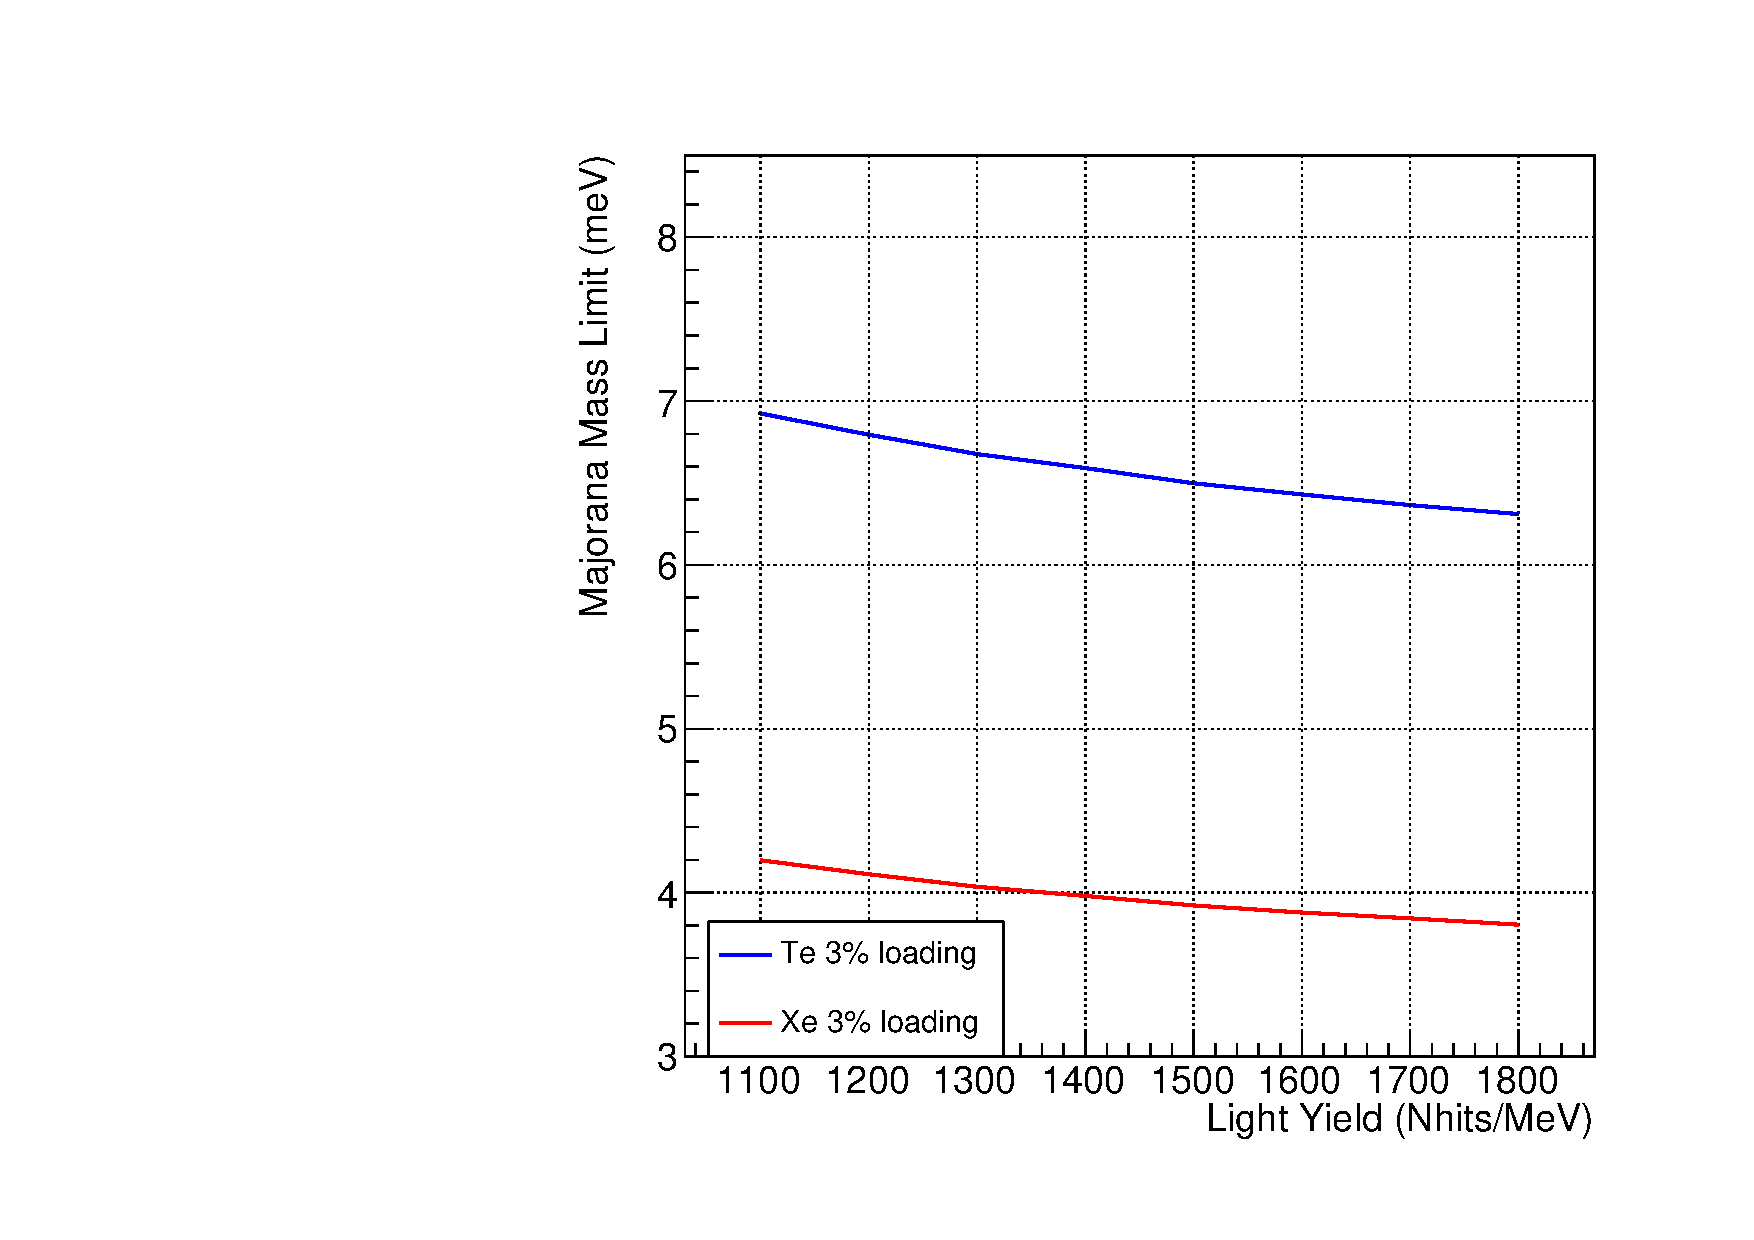
\includegraphics[width=\textwidth]{dbd/ly.pdf}
 \caption{Total detected light yield}
 \label{fig:scale-ly}
\end{subfigure}
\begin{subfigure}[b]{0.49\textwidth}
 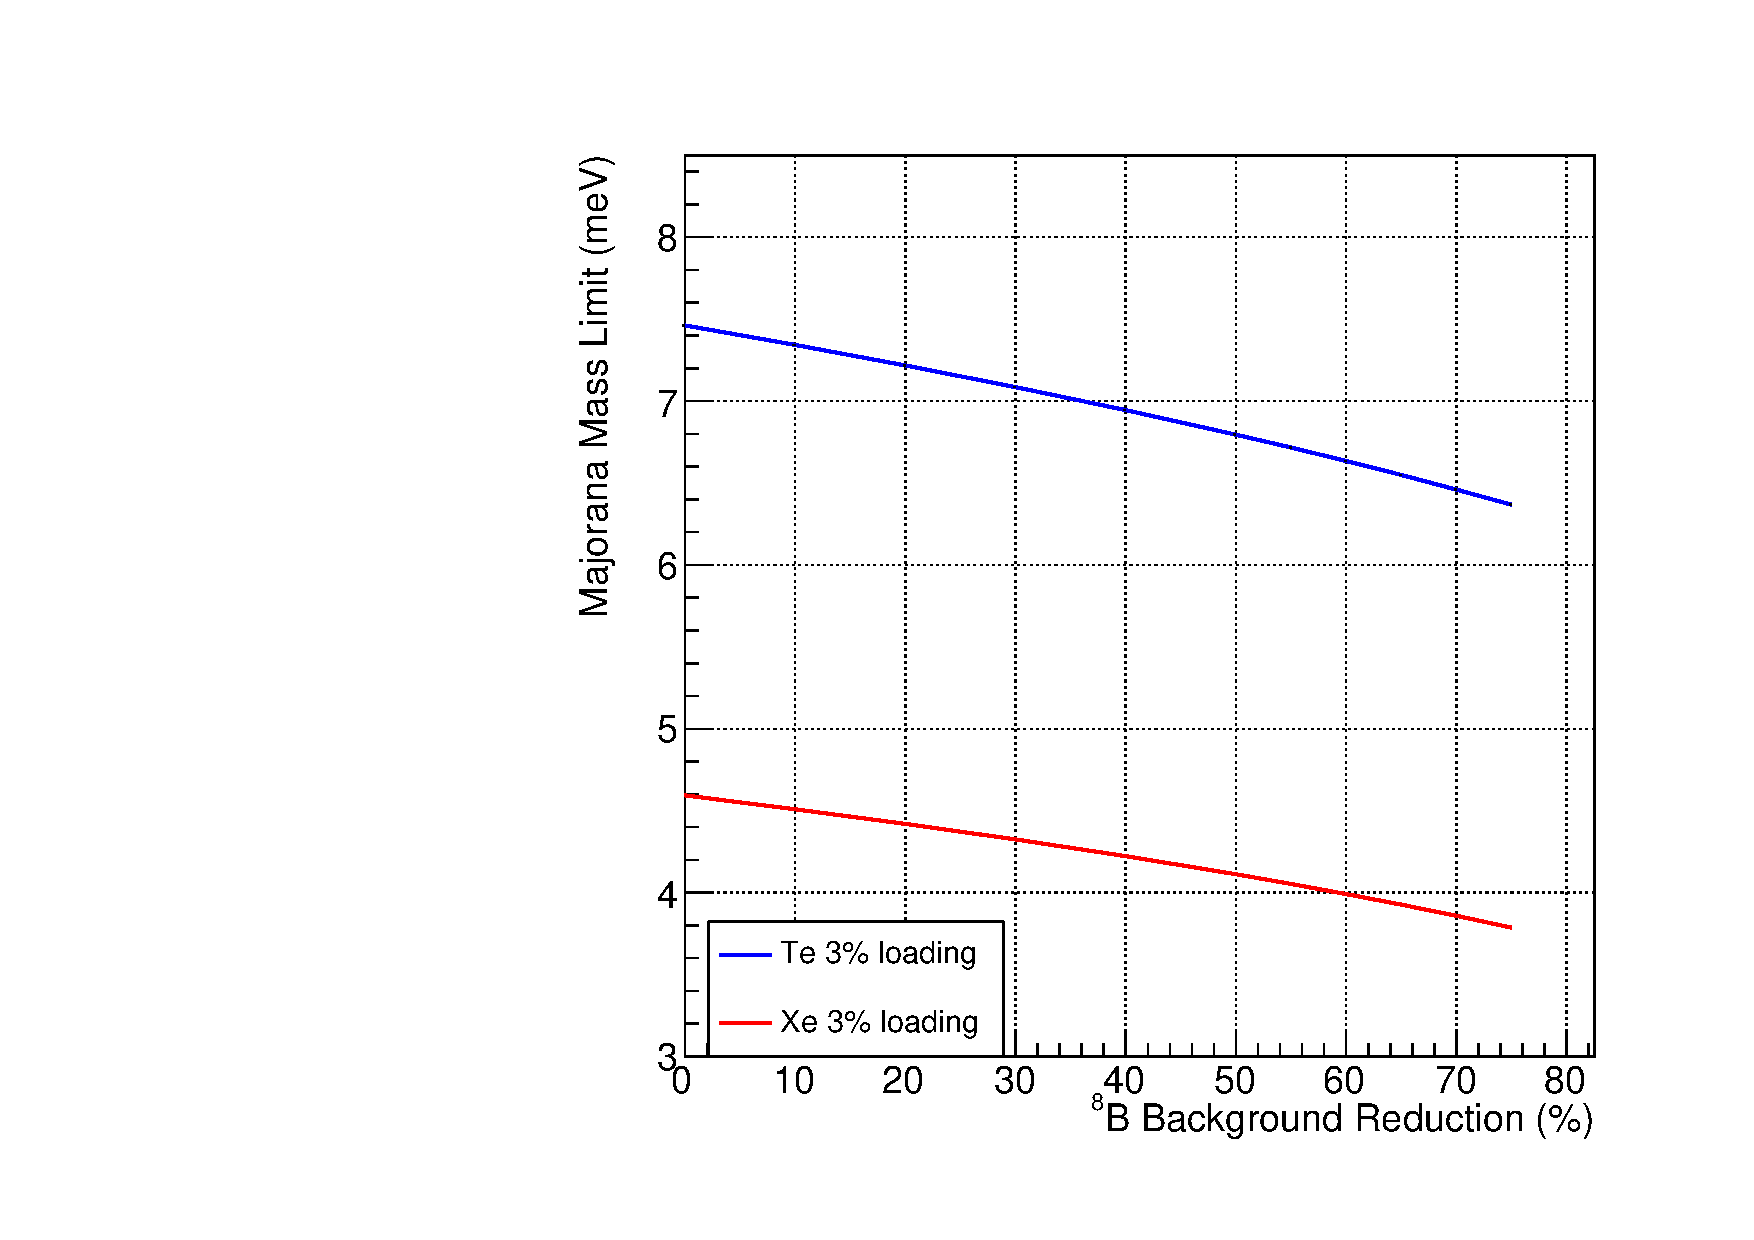
\includegraphics[width=\textwidth]{dbd/b8_reduction.pdf}
 \caption{Reduction factor for $^8$B solar neutrinos}
 \label{fig:scale-b8}
\end{subfigure}\\
\begin{subfigure}[b]{0.49\textwidth}
 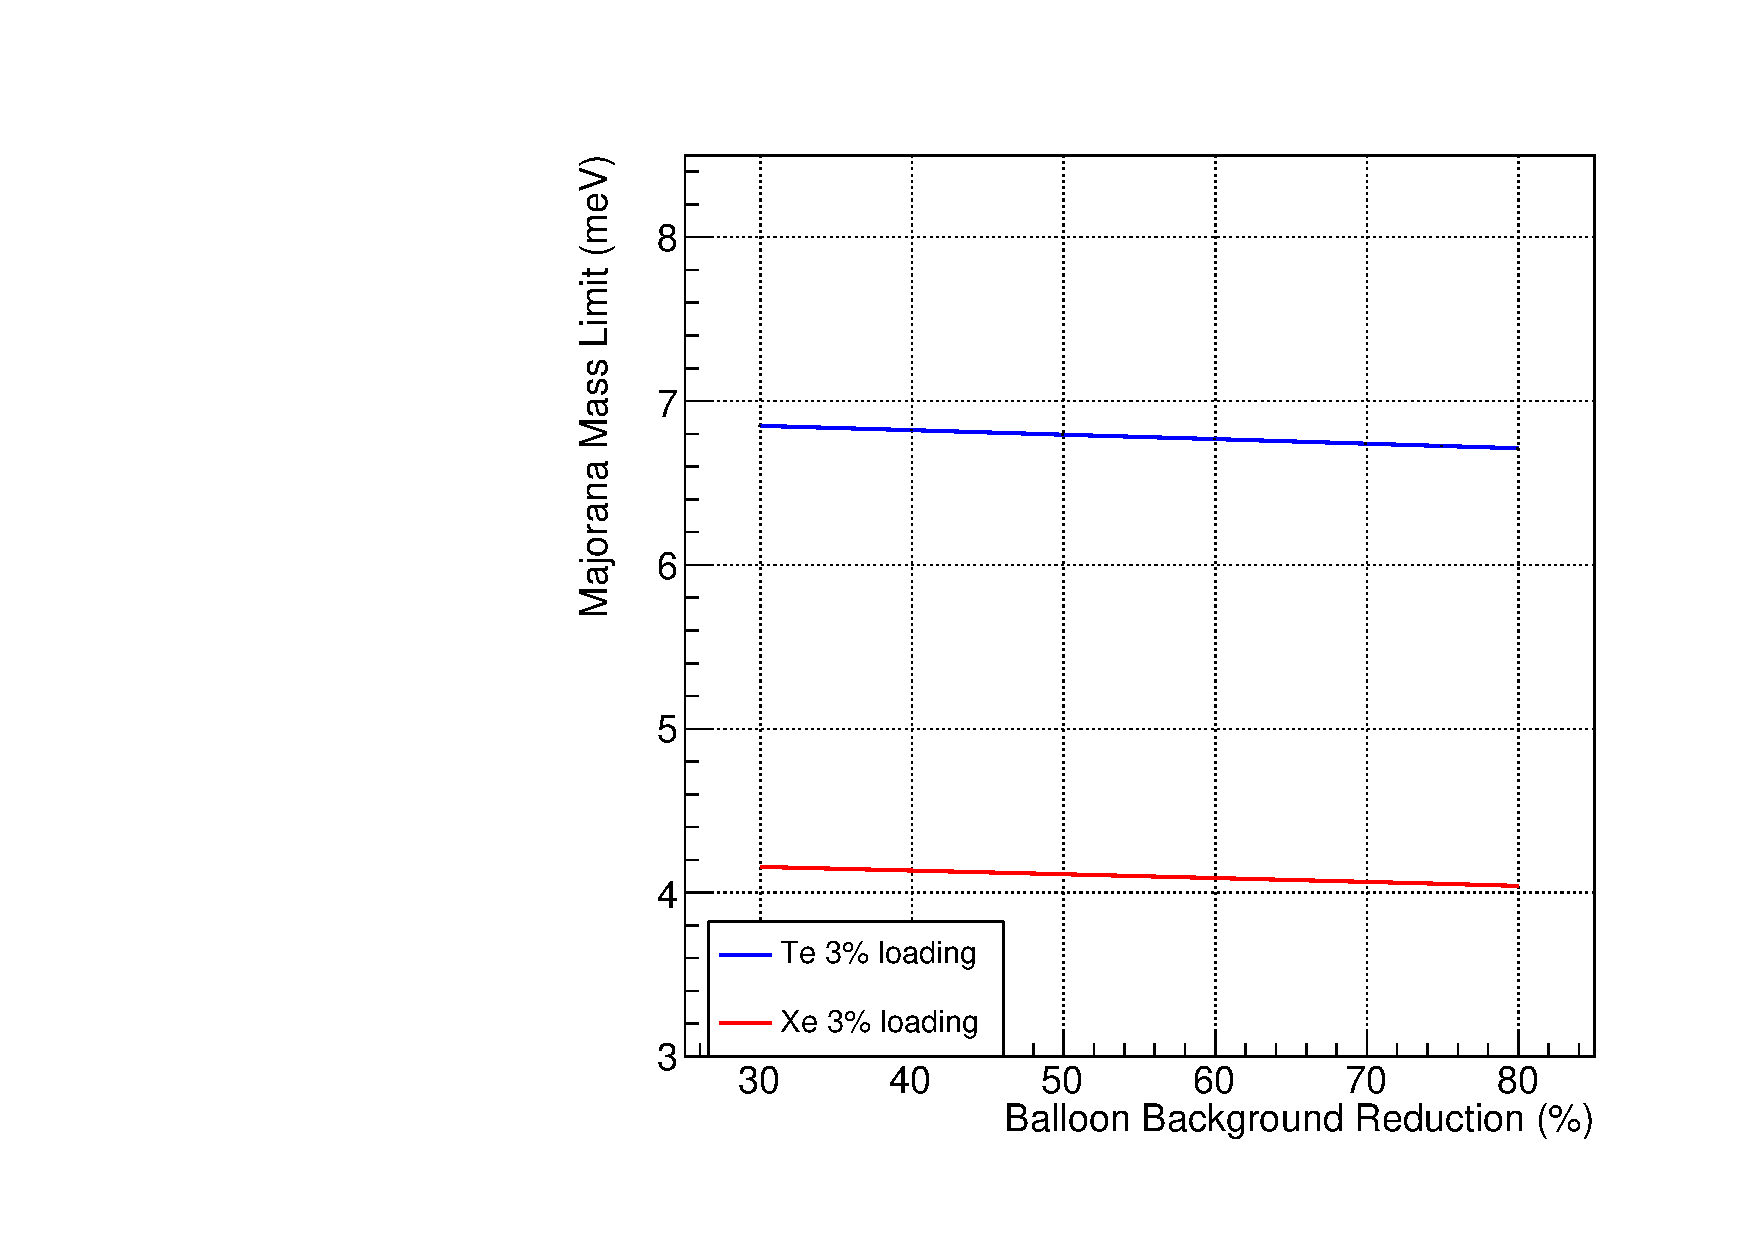
\includegraphics[width=\textwidth]{dbd/externals_reduction.pdf}
 \caption{Reduction factor for external backgrounds}
 \label{fig:scale-ext}
\end{subfigure}
\begin{subfigure}[b]{0.49\textwidth}
 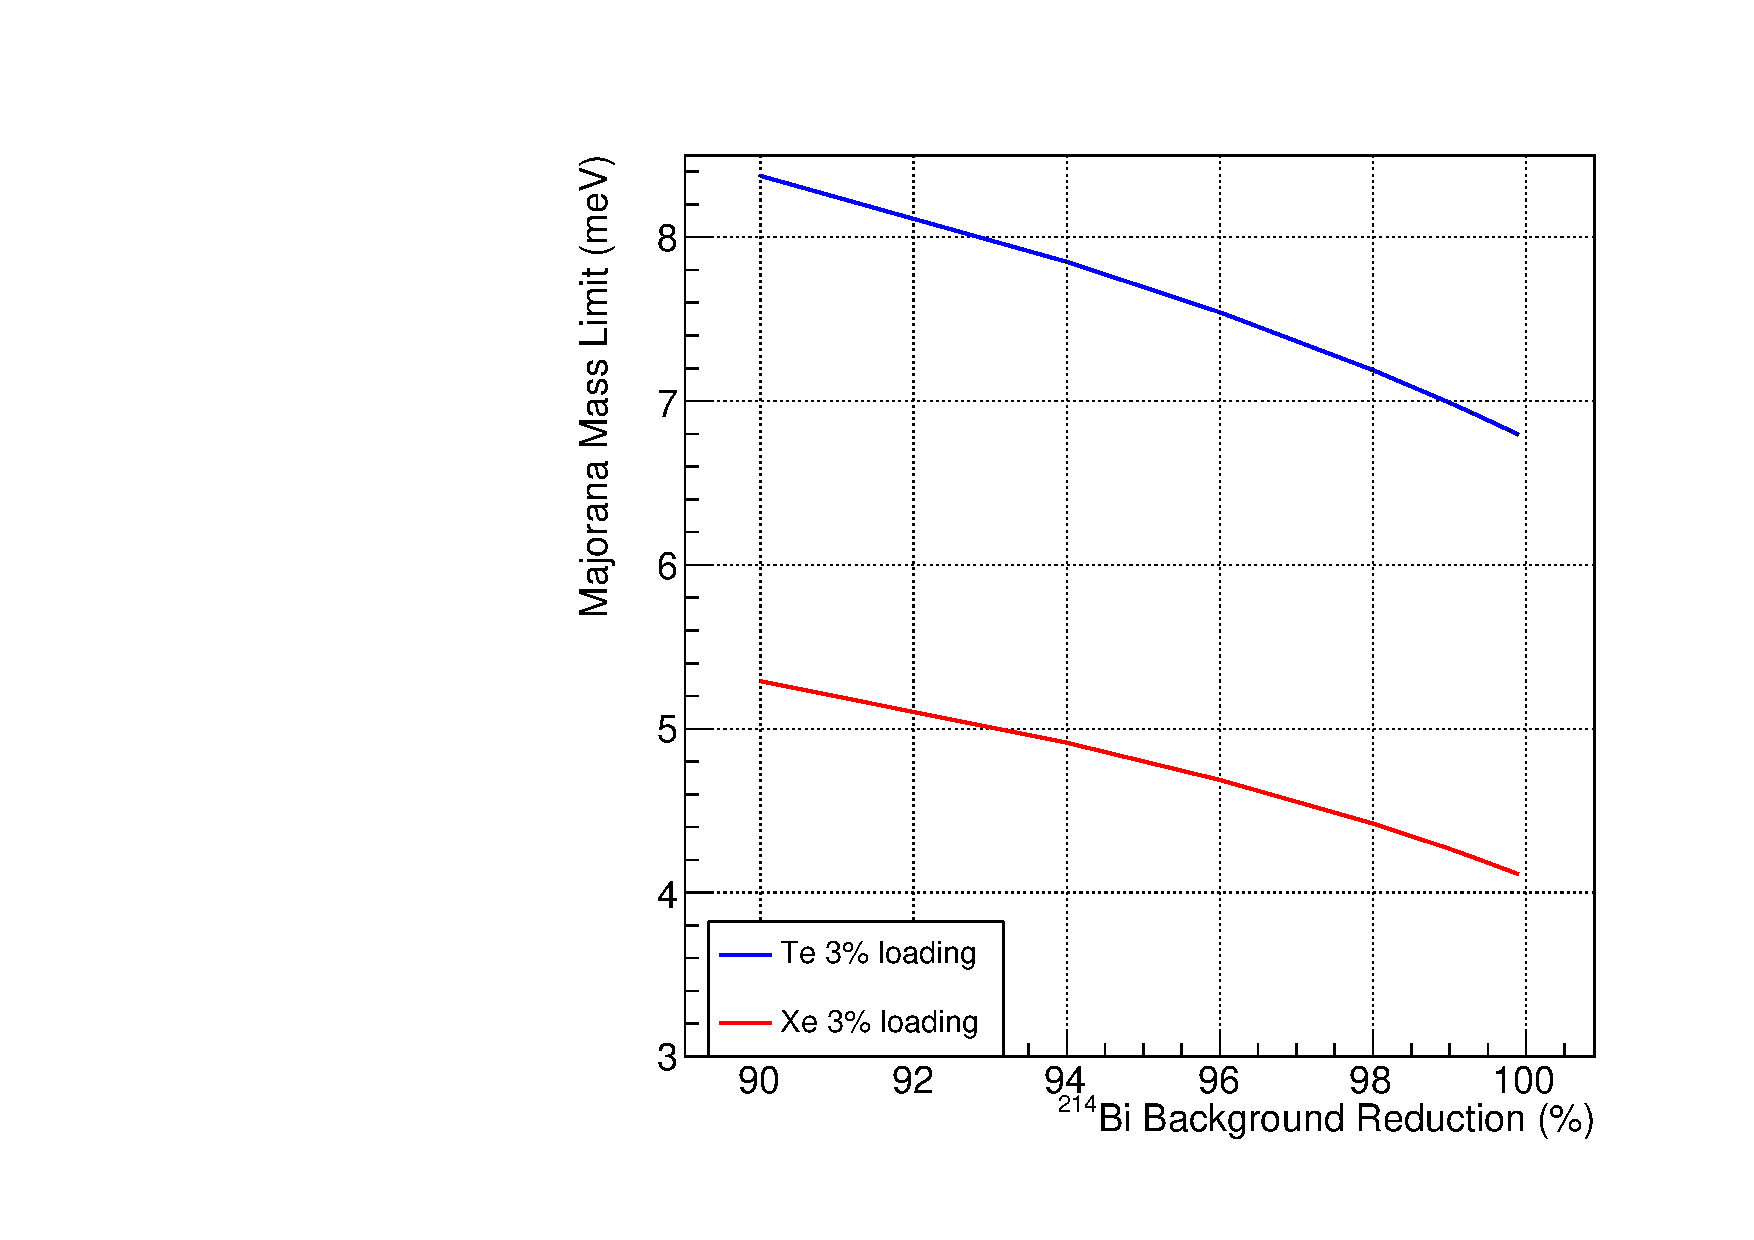
\includegraphics[width=\textwidth]{dbd/bi214_reduction.pdf}
 \caption{Reduction factor for $^{214}$Bi}
 \label{fig:scale-bi214}
\end{subfigure}
\caption{Mass sensitivity as a function of key experimental parameters.}
\label{fig:scaling-plots}
\end{figure}

\subsubsection{Conclusions}
In summary, the \textsc{Theia} experiment can perform a very sensitive search
for NLDBD, assuming a high level of Te or Xe loading and background levels
near those demonstrated by previous experiments. We have performed a
single-bin sensitivity analysis considering the dominant backgrounds for
an experiment located at the 4850 foot level of Homestake, accounting
for solar neutrino interactions, cosmogenic activation, and radioisotopic
contamination of detector materials. We have studied the behavior of these
backgrounds using a microphysical Monte Carlo simulation with a detector
model including scintillator and WbLS optics. We find that for aggressive
assumptions of radiopurity and background rejection, a \textsc{Theia} NLDBD
search is capable of reaching sensitivity within the non-degenerate normal
hierarchy parameter space.

%\section{Acknowledgements}
%
%\begin{thebibliography}{99}
%\bibitem{bxo16} N. Rossi, Neutrino 2016 Conference, London, 3---10 July 2016, \url{http://neutrino2016.iopconfs.org/IOP/media/uploaded/EVIOP/event_948/14.00__1_.pdf}
%\bibitem{mei09} D. M. Mei et al., Astropart. Phys. 31, 417–420 (2009).
%\bibitem{baudis15} L. Baudis et al., Eur. Phys. J. C 75, 485 (2015).
%\bibitem{zhang16} C. Zhang et al., Astropart. Phys. 84, 62--69 (2016).
%\bibitem{norm05} E. B. Norman et al., Nucl. Phys. B (Proc. Suppl.) 143, 508 (2005).
%\bibitem{bard97} D.W. Bardayan et al., Phys. Rev. C 55, 820 (1997).
%\bibitem{wang15} B.S. Wang et al., Phys. Rev. C 92, 024620 (2015).
%\bibitem{lozza15}  V. Lozza and J. Petzoldt, Astropart. Phys. 61, 62--71 (2015).
%\bibitem{snop16} S. Andringa et al., Advances in High Energy Physics 2016, 6194250 (2016).
%\bibitem{galb05} C. Galbiati, A. Pocar, D. Franco, A. Ianni, L. Cadonati, S. Schoenert, Phys.Rev. C 71 055805 (2005).
%\bibitem{gando16} Y Gando, Nuclear and Particle Physics Proceedings, vol. 273- 275, pp. 1842-1846 (2016).
%\bibitem{hagn00} T. Hagner et al., Astro. Phys. 14, 33--47, (2000).
%\bibitem{mei06} D. M. Mei and A. Hime, Phys. Rev. D 73, 053004 (2006).
%\bibitem{zbiri10} K. Zbiri, arxiv:0910.3714v3 [hep--ph] (2010).
%\bibitem{bxo2013} Borexino Collaboration, G. Bellini et al., JCAP08 49 (2013).
%\bibitem{SNO_3ph} SNO Collaboration, B. Aharmim et al., Physical Review C 88, 025501 (2013).
%\bibitem{Cuore017} C. Alduino et al., Eur. Phys. J. C 77 (2017).
%\bibitem{exo14}  J.B. Albert et al., Phys. Rev. C 89, 015502 (2014). 
%\bibitem{kam03} KamLAND Collaboration, K. Eguchi et al., Physical Review Letters 90, 021802, (2003).
%\bibitem{bxo09} Borexino Collaboration, C. Arpesella et al., Physical Review Letters 101,091302, (2008).
%\bibitem{gando13} A. Gando et al. Phys. Rev. Lett. 110, 062502 (2013).
%\bibitem{radiopurityorg} \url{https://www.radiopurity.org/rp/rp/_design/persephone/index.html?all}
%\bibitem{kamLAND_Zen} I. Shimizu, Frontiers of liquid Scintillator Technology (FroST16), March 18, 2016
%\url{https://indico.fnal.gov/getFile.py/access?contribId=45&sessionId=25&resId=0&materialId=slides&confId=10355}
%\bibitem{eijiri14} H. Ejiri and S. R. Elliott, Phys. Rev. C 89, 055501, (2014).
%\bibitem{eijiri17} H. Ejiri and S. R. Elliott, Phys. Rev. C 95, 055501 (2017).
%\bibitem{decay0} O.A.Ponkratenko, V.I.Tretyak, Yu.G.Zdesenko, Phys. At. Nucl. 63, 1282   (2000)  (nucl-ex/0104018)
%\bibitem{2012PhRvC..85c4316K} Kotila, J., \& Iachello, F. (2012). Phase-space factors for double-$\beta$ decay. Physical Review C - Nuclear Physics, 85(3), 034316. http://doi.org/10.1103/PhysRevC.85.034316
%\bibitem{Barea:2013wb} Barea, J., Kotila, J., \& Iachello, F. (2013). Nuclear matrix elements for double-$\beta$ decay. Physical Review C - Nuclear Physics, 87(1).
%\end{thebibliography}
%
%%\bibliographystyle{alpha}
%%\bibliography{sample}
%
%\end{document}




\section{Physics Sensitivities and Detector Requirements}\label{s:physics}

\textsc{Theia} would address a broad program of physics, including: geo-neutrinos, supernova neutrinos, 
nucleon decay, measurement of the neutrino mass hierarchy and CP violating phase, 
and even a next-generation NLDBD search.   


%\subsection{High-Energy Physics}
%\subsubsection{Detector Simulation - \bf volunteers?}
%Summary of simulation used in following sections, including e.g. high energy physics list, specific parameters for each detector configuration.

\subsubsection{Long Baseline - M Wilking for LBL group}
\paragraph{Motivation}
BRIEF intro to physics motivation, and status of the field: our major competitors
\paragraph{XX with THEIA}
What we bring to the table - pros of THEIA design \newline
Sensitivity estimates with baseline design (one of THEIA i--iii)
\paragraph{Detector Requirements}
A summary of the impact of different detector choices i.e. what happens if we stray from the relevant baseline


\subsection{Nucleon Decay - \bf volunteers?}
\paragraph{Motivation}
BRIEF intro to physics motivation, and status of the field: our major competitors
\paragraph{XX with THEIA}
What we bring to the table - pros of THEIA design \newline
Sensitivity estimates with baseline design (one of THEIA i--iii)
\paragraph{Detector Requirements}
A summary of the impact of different detector choices i.e. what happens if we stray from the relevant baseline

\subsection{Atmospheric Neutrinos - \bf volunteers?}
\paragraph{Motivation}
BRIEF intro to physics motivation, and status of the field: our major competitors
\paragraph{XX with THEIA}
What we bring to the table - pros of THEIA design \newline
Sensitivity estimates with baseline design (one of THEIA i--iii)
\paragraph{Detector Requirements}
A summary of the impact of different detector choices i.e. what happens if we stray from the relevant baseline

%\subsection{Low-Energy Physics}
%\subsubsection{Detector Simulation - \bf volunteers?}
%Summary of simulation used in following sections, including e.g. high energy physics list, specific parameters for each detector configuration.

\subsection{Neutrinoless Double Beta Decay - L Winslow, V Lozza, A Mastbaum for DBD group}
%\paragraph{Motivation}
%BRIEF intro to physics motivation, and status of the field: our major competitors
%\paragraph{XX with THEIA}
%What we bring to the table - pros of THEIA design \newline
%Sensitivity estimates with baseline design (one of THEIA i--iii)
%\paragraph{Detector Requirements}
%A summary of the impact of different detector choices i.e. what happens if we stray from the relevant baseline

%\documentclass[a4paper]{article}
%
%%% Language and font encodings
%\usepackage[english]{babel}
%\usepackage[utf8x]{inputenc}
%\usepackage[T1]{fontenc}
%\usepackage[noadjust]{cite}
%\usepackage{booktabs}
%\usepackage{subcaption}
%\renewcommand{\citedash}{--}  
%%% Sets page size and margins
%\usepackage[a4paper,top=3cm,bottom=2cm,left=3cm,right=3cm,marginparwidth=1.75cm]{geometry}
%
%%% Useful packages
%\usepackage{amsmath}
%\usepackage{url}
%\usepackage{graphicx}
%%\usepackage[colorinlistoftodos]{todonotes}
%\usepackage[colorlinks=true, allcolors=blue]{hyperref}
%
%\title{\textsc{Theia} DBD White Paper}
%%\author{T. Klosterman, V. Lozza, A. Mastbaum}
%
%\begin{document}
%\maketitle

%\section{Introduction}
The \textsc{Theia} search for neutrinoless double beta decay (NLDBD) aims for
sensitivity to the non-degenerate normal hierarchy parameter space
within the canonical framework of light Majorana neutrino exchange and
three-neutrino mixing, at the level of $m_{\beta\beta}\sim5$ meV.
This is achieved through the loading of a very large
mass of a NLDBD candidate isotope into an ultra-pure liquid scintillator
target, together with coincidence and topological particle identification
techniques.

\subsubsection{Detector Configuration}

For the present studies, we model the detector as a cylinder with a 20\,m fiducial radius and a 40\,m height, for a total fiducial mass of 50\,kt, with a PMT coverage of 90\%. The detector is assumed to be located in the Homestake mine, at a depth of 4300\,m.w.e. The double-beta decay isotope under investigation is loaded into a nylon balloon of 435\,$\mu$m thickness and 8\,m radius, filled with ultra-pure liquid scintillator (LAB + 2\,g/l PPO for a density of 0.86 g/cm$^3$). The volume outside the balloon is filled with a WbLS (10\% LAB-PPO and 90\% water). We investigate two major loading cases: 3\% enriched Xenon (89.5\% in $^{136}$Xe) and 5\% natural Tellurium (34.1\% in $^{130}$Te).

The optical properties of the unloaded LAB+PPO cocktail have been measured by the SNO+ collaboration, while those of the WbLS are obtained by weighting contributions of the LAB+PPO and water, and are consistent with benchtop measurements. As a baseline, an average light yield of 1200 PMT hits per deposited MeV is assumed (corresponding to about 3\%/$\sqrt(E)$ energy resolution). This value includes the reduction in the light yield due to the addition of the isotope, estimated to be around 30\% at 5\%, or higher, loadings. For the specific case of Xe loaded scintillator, the used light yield is likely an underestimation as the KamLAND-Zen experiment predicts a reduction of only 15\% at the reached 3\% loading, corresponding to 1530 Nhits/MeV \cite{KZ-2011}. Figure \ref{fig:scale-ly} shows the impact of the light yield on the THEIA sensitivity. 
Simulations are obtained with the Geant4-based RAT-PAC software package \footnote{\url{https://github.com/rat-pac/rat-pac}}, part of the radioactive decays are simulated using the Decay0 code \cite{decay0}. Reconstructed energy is approximated by assuming the Poisson limit of
photon counting: the true deposited energy, accounting for quenching, is smeared out by a Gaussian resolution function corresponding to the light
yield.

\subsubsection{Backgrounds}

\begin{table}[t]
\centering
\scalebox{0.9}{
\begin{tabular}{lcccc}
\toprule
{\bf Source} & {\bf Target level} & {\bf Expected events/y}   & \multicolumn{2}{c}{\bf Events/ROI$\cdot$y} \\
& & & 5\% $^{nat}$Te  & 3\% $^{enr}$Xe  \\
\midrule
Balloon $^{10}$C  & & 500 &  2.5       & 2.5\\
$^{8}$B neutrinos (normalization from \cite{SNO_3ph}) &  & 2950   & 13.8      & 13.8  \\
$^{130}$I (Te target)  &  & 155  (30 from $^{8}$B) & 8.3 & - \\
%$^{136}$Cs (Xe target) &   & 47 (6 from $^{8}$B)   & &\\
$^{136}$Cs ($^\mathrm{enr}$Xe target) & & 478 (68 from $^{8}$B) & -&0.06\\
2$\nu\beta\beta$ (Te target, T$_{1/2}$ from \cite{Cuore017}) &   & 1.2$\times$10$^{8}$  & 8.0       &  -\\  
%2$\nu\beta\beta$ (Xe target,  T$_{1/2}$ from \cite{gando16, exo14})  & & 7.0$\times$10$^{6}$  & & \\  
2$\nu\beta\beta$ ($^\mathrm{enr}$Xe target, T$_{1/2}$ from \cite{gando16, exo14}) &  &  7.1$\times$10$^{7}$  &   -    & 3.8  \\  
Liquid scintillator & $^{214}$Bi: $10^{-17}$ g$_{U}$/g  & 7300 & 0.4        & 0.4\\
   & $^{208}$Tl: $10^{-17}$ g$_{Th}$/g  & 870  & -& -\\
Nylon Vessel  \cite{radiopurityorg, kamLAND_Zen}  & $^{214}$Bi: $<1.1\times10^{-12}$ g$_{U}$/g & 1.2$\times$10$^{5}$   & 2.4       & 2.7   \\
 & $^{208}$Tl: $<1.6\times10^{-12}$ g$_{Th}$/g   & 2.1$\times$10$^{4}$  & 0.03       & 0.01  \\
%PMTs  & $^{214}$Bi: $10^{-6}$ g$_{U}/$PMT  &  &&  \\
 %& $^{208}$Tl: $10^{-6}$ g$_{Th}/$PMT  & && \\
% {\bf Total}      &&         & 35.5      & 23.5      \\
\bottomrule
\end{tabular}}
\caption{Dominant background sources expected for the NLDBD search in \textsc{Theia}. The assumed loadings are 3\% for Xe, for a $^{136}$Xe mass of 49.5\,t, and 5\% for Te, for a $^{130}$Te mass of  31.4\,t. The events in the ROI/yr are given for a fiducial volume of 7\,m and an symmetric energy range around the Q-value of the reaction (\textit{see text}). A rejection factor of 92.5\% is applied to $^{10}$C, of 99.9\% to $^{214}$Bi, of 50\% to the balloon backgrounds, and of 50\% to the $^8$B solar neutrinos.}
\label{tab::bckg}
\end{table}

The main sources of background included in the this analysis are summarized in Table \ref{tab::bckg} and described below:

\begin{description}
\item[Double Beta Decay] This irreducible background is due to the $2\nu\beta\beta$ decays of $^{130}$Te or $^{136}$Xe. Due to the steeply-falling
spectrum, the number of events falling in the ROI depends strongly on the energy resolution.
\item[Cosmogenic Production] These backgrounds are due to activation of nuclei by muons (during data taking) or protons and neutrons (during material production and handling at Earth's surface). The neutron and proton production's rates in Xe and Te has been investigated by several authors \cite{mei09, baudis15, zhang16, norm05, bard97, wang15, lozza15}. Among the most important nuclides there are $^{60}$Co ($Q=2.8$ MeV, $T_{1/2}=5.27$ y) and $^{110m}$Ag ($Q=3.1$ MeV, $T_{1/2}=250$ d). Mitigation of these background sources requires minimal exposure at sea level, a deep underground cool-down period, chemical purification processes \cite{snop16}, and, to limit the in-situ production during data taking, the use of a water shield. In these studies, it is assumed that proper measures are taken to handle the target material, reducing the background to a negligible level. For what concerns the in-situ muon induced background, the most dangerous nuclide for the NLDBD study is $^{10}$C ($Q=3.65$ MeV, $T_{1/2}=19.3$ s) produced by muon interaction with the carbon atoms of the liquid scintillator. The estimated event's rate is about 300 events/kt/yr \cite{hagn00} for a muon flux of $4.2\times10^{-9}$ cm$^{-2}$ s$^{-1}$ and an average muon energy of 293\,GeV \cite{mei06}. A reduction of 92.5\% of the $^{10}$C background has been demostrated by Borexino \cite{bxo2013}, using a three-fold coincidence technique\cite{galb05, gando16}. An alternative approach could be using machine learning, as described in the reconstruction section. However, a rejection of at least 90\% is required in order to maintain a sensitivity down to the normal hierarchy.
\item[Solar Neutrinos] $^{8}$B solar neutrino elastic scattering in the target material results in a background that is approximately flat across the NLDBD energy region of interest. Figure \ref{fig:scale-b8} shows the sensitivity scaling with solar neutrino event's reduction. A rejection of at least 50\% is requested in order to reach the sensitivity goal. MonteCarlo simulations show that, for 2.5\,MeV electrons in water, about 80\% of the $^{8}$B events can be rejecting keeping a 75\% acceptance for the neutrinoless double-beta decay signal (assumed to be isotropic). The use of high quantum efficiency PMTs, together with a large coverage, is expected to improve this value. On the other hand, the scintillation light is a confounding factor (in slow scintillator it might be harder to reach the purity requirements), which might reduce the discrimination. Nevertheless, a 50\% rejection is considered an achievable value. This is further shown in \cite{elagin19}, where more than 50\% rejection in $^{8}$B is achieved, retaining more than 70\% of the signal.
Another background induced by solar neutrinos (mainly $^{8}$B and $^{7}$Be) are high Q-value nuclides produced by charged current interaction with $^{130}$Te and $^{136}$Xe \cite{eijiri14, eijiri17}. Due to their long half life, a tagging technique based on a delayed coincidence is expected to have a small efficiency. 
\item[Internal Contamination:] $^{214}$Bi ($Q=3.27$ MeV, U-chain) and $^{208}$Tl ($Q=5$ MeV, Th-chain) decays can fall in the energy window used for the NLDBD studies. The targeted scintillator cocktail purity for the \textsc{Theia} experiment is 10$^{-17}$ g/g in both U and Th. Liquid scintillator purities better than $\times$ 10$^{-18}$ g/g in U and Th have been obtained in the Phase-II of Borexino \cite{bxo16}, while KamLAND-Zen, has reached a cleanliness of the order of $\times$ 10$^{-16}$ g/g U for the 3\% loaded case \cite{gando13}. The targeted purity is considered achievable by improving the target material purification technique, i.e the purity grade of the chemicals used to process the tellurium. In addition delayed coincidence techniques can further reduce the number of $^{214}$Bi decays falling in the ROI. A rejection better than 99.95\% for the $^{214}$BiPo in the ROI has been shown by the KamLAND-Zen experiment \cite{KD-Zen}, while Monte Carlo studies for the SNO+ experiment show that the rejection in the double-beta decay region can be as high as 99.99\% \cite{snop16}. For the aimed target purity, it is required that the $^{214}$Bi is further reduced by 99.9\%. Larger reduction factors have a minimum effect on the overall sensitivity.
\item[External Sources:] Decays from U and Th-chain impurities present in the balloon material, the external water-based liquid scintillator, the
shielding water, and in the PMTs also contribute to the background. External background events can be reduced using a fiducial volume cut, and hit time information. In the following study a rejection factor of 50\%, on the top of the fiducial volume, is assumed. However, a smaller reduction factor won't affect the sensitivity.
\end{description}

\subsubsection{NLDBD Sensitivity: Counting Analysis}\label{sec::sensitivity}

To estimate the sensitivity, a single-bin counting analysis is employed. Since all backgrounds do not scale with isotope mass (e.g. solar neutrinos
and external $\gamma$ backgrounds), we use the Monte Carlo to evaluate the background expectation, establish a confidence region using the Feldman-Cousins frequentist approach, and derive an expected limit on the NLDBD half life:
\begin{equation}
\label{eq:sens}
\widehat{T}_{1/2}^{0\nu\beta\beta}(\alpha) = 
\frac{N\cdot \epsilon \cdot t \cdot \ln 2}{\mathrm{FC}(n=b, b; \alpha)}
%\widehat{T}_{1/2}^{0\nu\beta\beta}(\alpha) = \left\langle
%\frac{n\cdot \epsilon \cdot t \cdot \ln 2}{\mathrm{FC}(N, b; \alpha)}
%\right\rangle_{n=\mathrm{Pois}(b)}
\end{equation}
where $N$ is the number of atoms of active NLDBD isotope, $\epsilon$ is the efficiency, $t$ the live time, and $b$ the expected background.
`FC' refers to a Feldman-Cousins interval at confidence level $\alpha$.

The expected event rates per year for a $^\mathrm{nat}$Te or $^\mathrm{enr}$Xe loaded \textsc{Theia} detector are given in Table \ref{tab::bckg}, for a fiducial volume is 7\,m (67\%) and an asymmetric energy region,  from $-\sigma/2 \to 2\sigma$, to maximize signal acceptance ($\epsilon=66.9$\%) while removing much of the steeply-falling two-neutrino DBD background spectrum. Figure \ref{fig:spectrum-plots} shows the background spectra near the endpoint in the Te (Figure \ref{fig:spectrum-te}) and Xe (Figure \ref{fig:spectrum-xe}) cases.

The expected sensitivity (90\% CL sensitivity), using phase space factors from \cite{2012PhRvC..85c4316K} and matrix element from \cite{Barea:2013wb} (g$_{A}$=1.269) is:
\begin{eqnarray*}
\mathrm{\bf Te:}~~
  T_{1/2}^{0\nu\beta\beta} > 1.5\times10^{28}~\mathrm{y},~
  m_{\beta\beta} < 5.4~\mathrm{meV}\\
  \mathrm{\bf Xe:}~~
  T_{1/2}^{0\nu\beta\beta} > 2.7\times10^{28}~\mathrm{y},~
  m_{\beta\beta} < 4.8~\mathrm{meV}
\end{eqnarray*}

It should be noted that for the case of Xenon, the use of a more realistic light yield of about 1500\,nhits/MeV, as obtained from  \cite{KZ-2011}, would increase the half-life limit to 3$\times 10^{28}$ years, corresponding to a $m_{\beta\beta} < 4.6~\mathrm{meV}$. Unfortunately, the required mass of Xe to reach the normal hierarchy is about 10 times the world annual production, which makes the use of Xe likely impractical.

%\begin{table}
%\centering
%\begin{tabular}{ccc}
%\toprule
%                          & \multicolumn{2}{c}{\bf Events/ROI$\cdot$y} \\
%{\bf Signal}              & Te Loading & $^{enr}$Xe Loading \\
%Loaded isotope mass [t] & 31.4 & 49.5 \\
%\midrule
%$0\nu\beta\beta$ (10 meV) & 108.9       & 116.4      \\
%\midrule
%$2\nu\beta\beta$          & 80.0       & 38.2       \\
%$^8$B Solar ES  (50\%)           & 138.5      & 138.4      \\
%$^{10}$C  (92.5\%)                & 24.6       & 25.4       \\
%$^{130}$I                 & 80.5       & ---        \\
%$^{130m}$I                & 2.9        & ---        \\
%$^{136}$Cs                & ---        & 0.57       \\
%$^{208}$Tl                & 0.02       & 0.002      \\
%$^{214}$Bi  (99.9\%)               & 4.0        & 4.4        \\
%Balloon $^{214}$Bi  (50\%)       & 24.0       & 27.4       \\
%Balloon $^{208}$Tl  (50\%)      & 0.25       & 0.14       \\
%\midrule
%{\bf Total}               & 354.8      & 234.5      \\
%\bottomrule
%\end{tabular}
%\caption{Expected background counts per year in the ROI. In parenthesis is shown the reduction factor applied.}
%\label{tab:counts}
%\end{table}

\begin{figure}
\centering
\begin{subfigure}[b]{0.35\textwidth}
 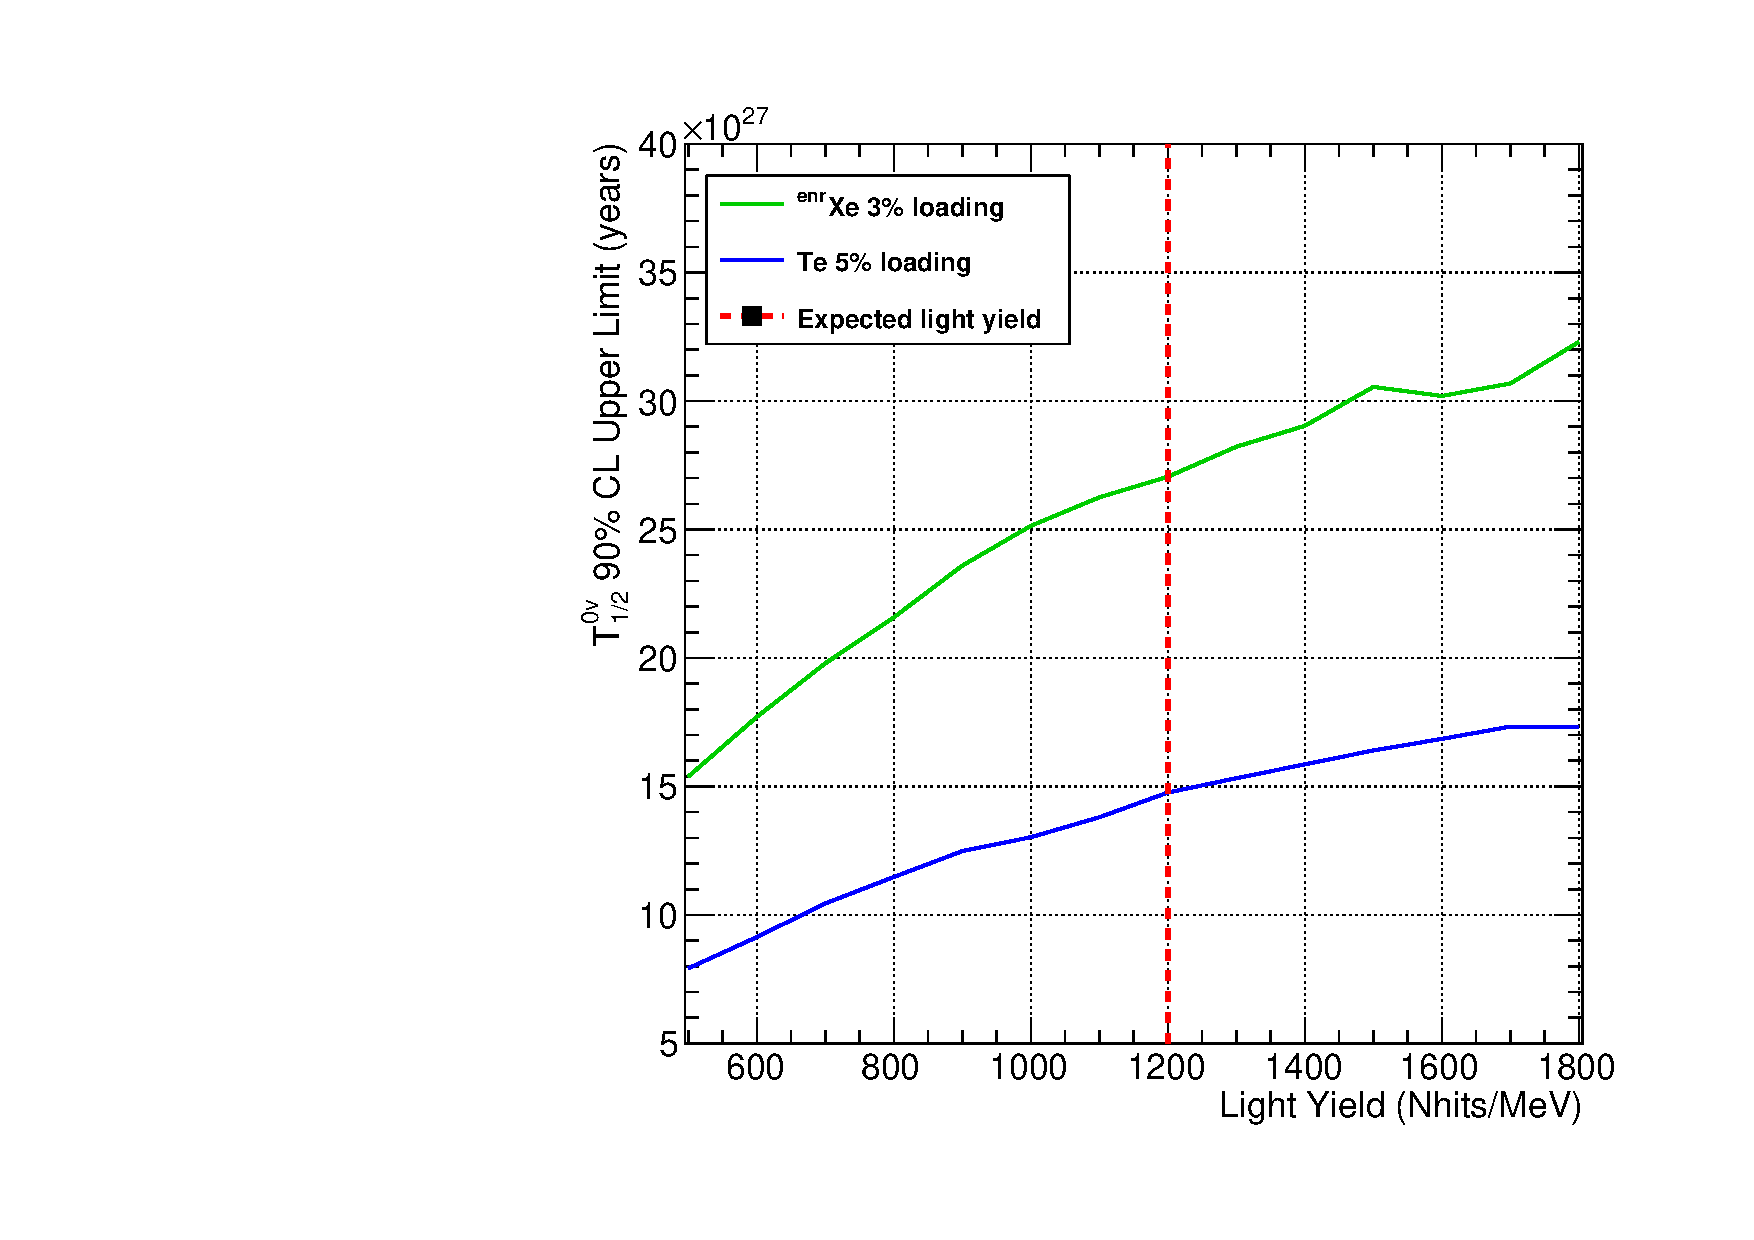
\includegraphics[width=\textwidth]{dbd/ly_comparison_lifetime_500.pdf}
 \caption{Light yield}
 \label{fig:scale-ly}
\end{subfigure}
\begin{subfigure}[b]{0.35\textwidth}
 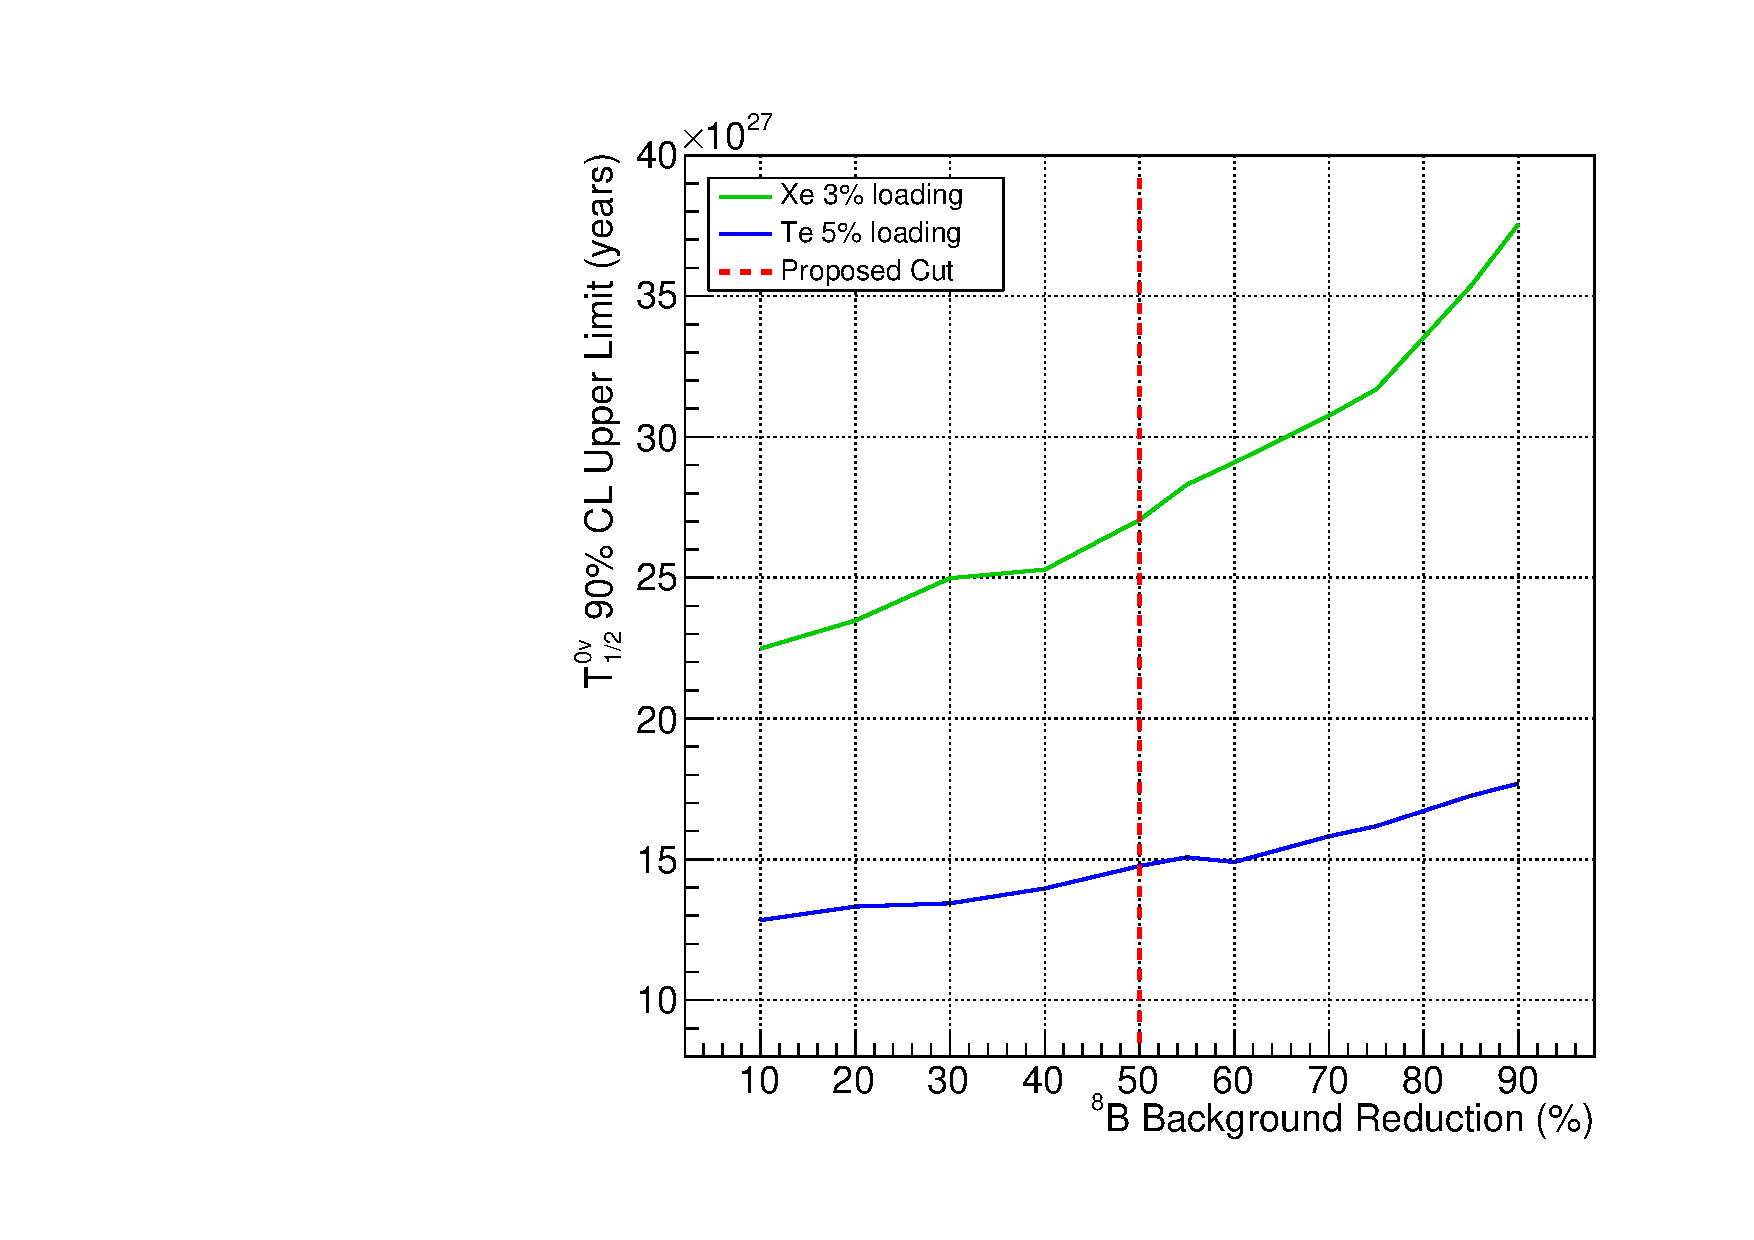
\includegraphics[width=\textwidth]{dbd/b8_reduction_fc.pdf}
 \caption{$^8$B solar neutrinos' reduction}
 \label{fig:scale-b8}
\end{subfigure}\\
%\begin{subfigure}[b]{0.33\textwidth}
% 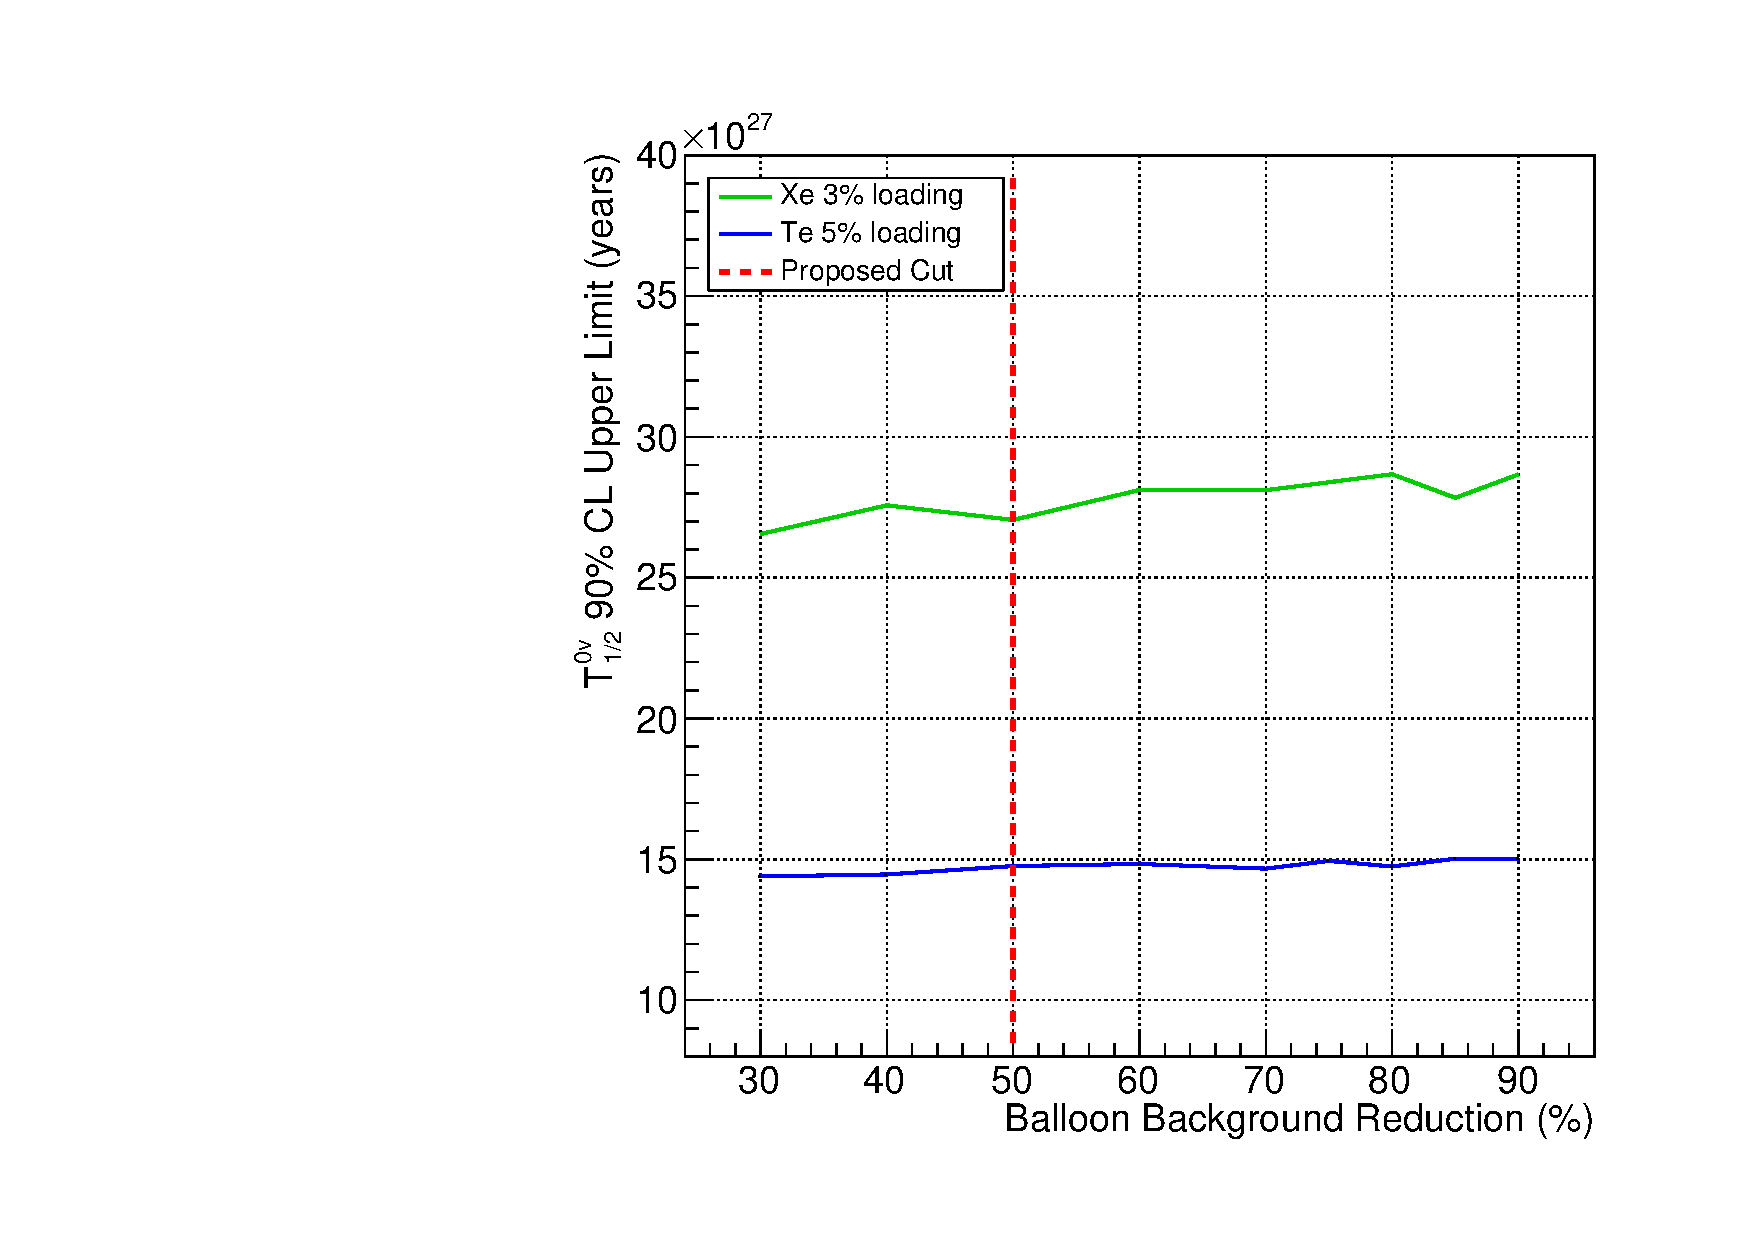
\includegraphics[width=\textwidth]{dbd/externals_reduction_fc.pdf}
% \caption{Reduction factor for external backgrounds}
% \label{fig:scale-ext}
%\end{subfigure}
%\begin{subfigure}[b]{0.35\textwidth}
% 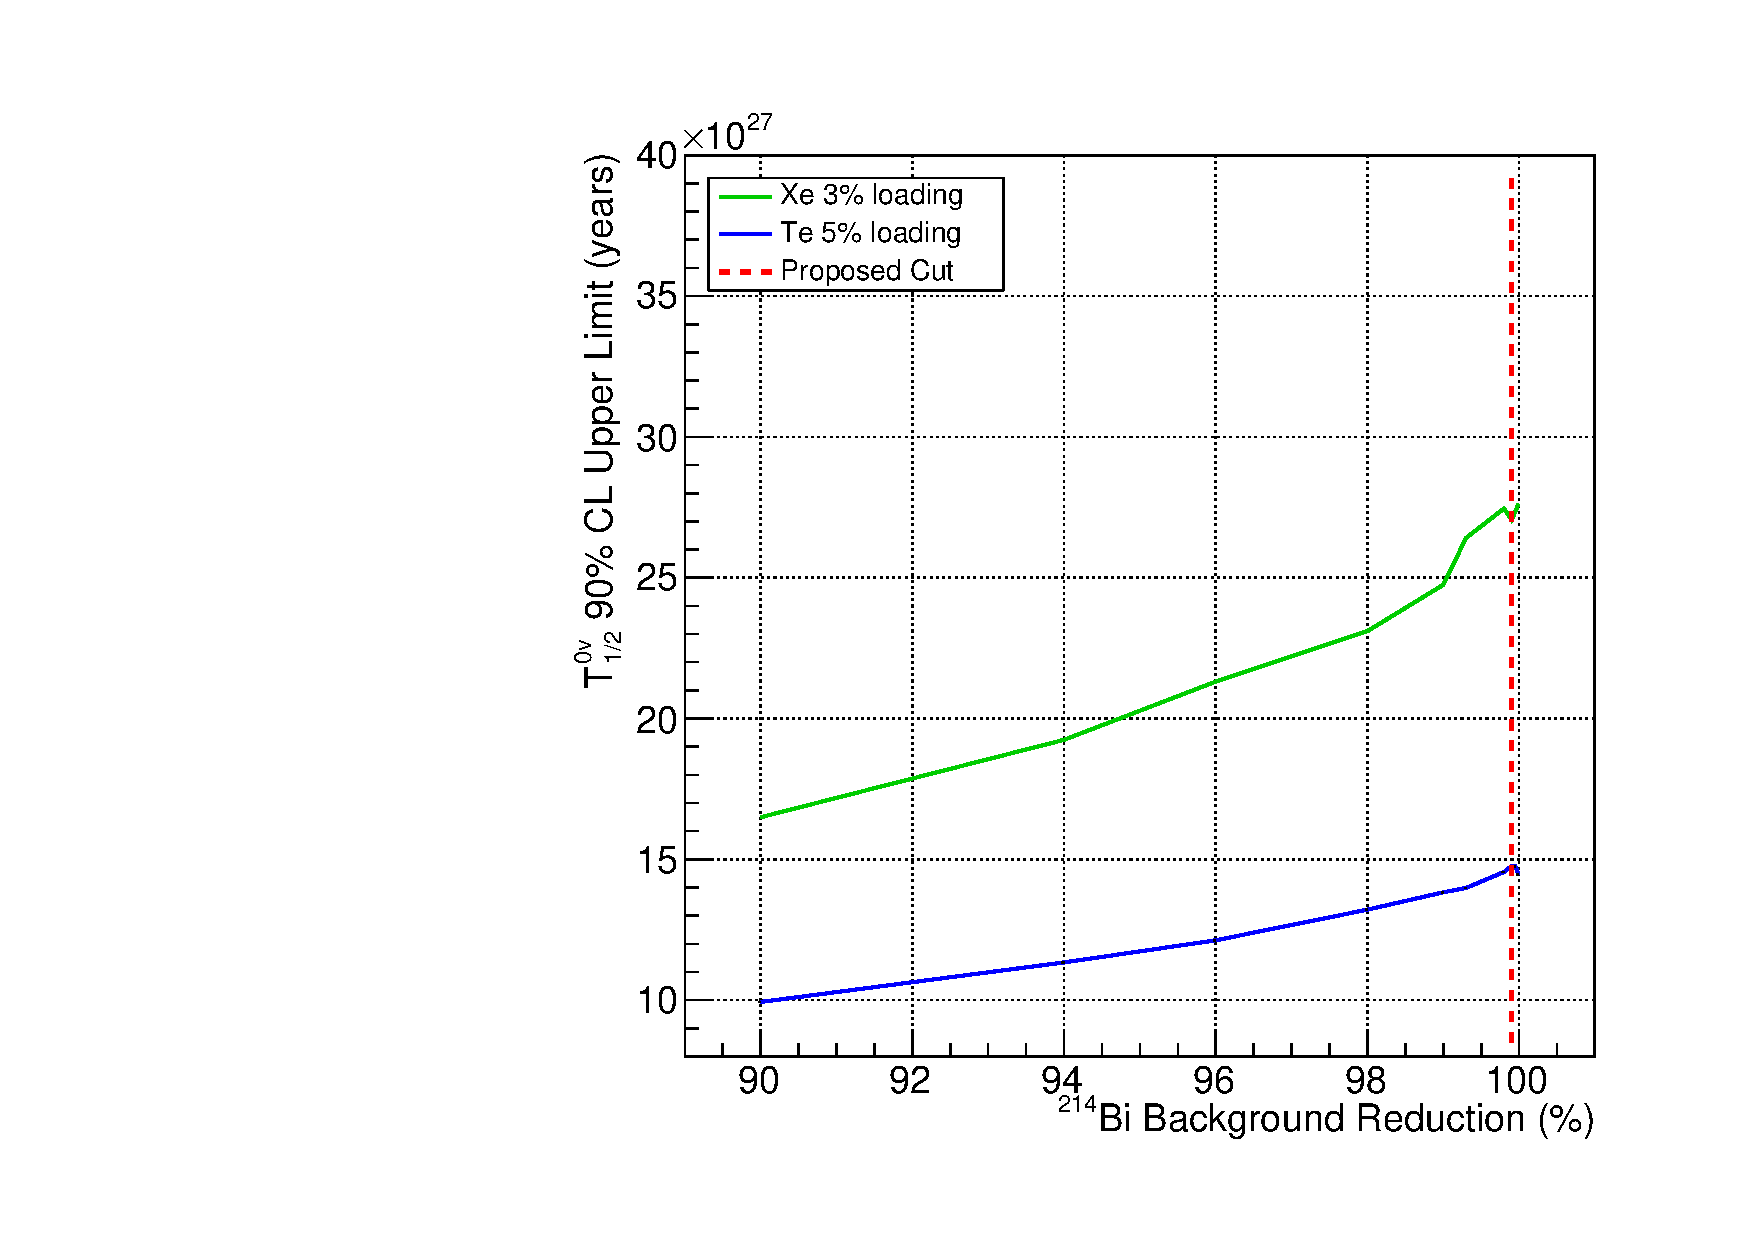
\includegraphics[width=\textwidth]{dbd/bi214_reduction_fc.pdf}
% \caption{Reduction factor for $^{214}$Bi}
% \label{fig:scale-bi214}
%\end{subfigure}
\caption{Mass sensitivity as a function of key experimental parameters. The vertical dashed red lines show the values used in the analysis. For the same detector optical properties, a variation in the light yield corresponds to a scaling on the PMT coverage.}
\label{fig:scaling-plots}
\end{figure}

\begin{figure}
\centering
\begin{subfigure}[b]{0.45\textwidth}
 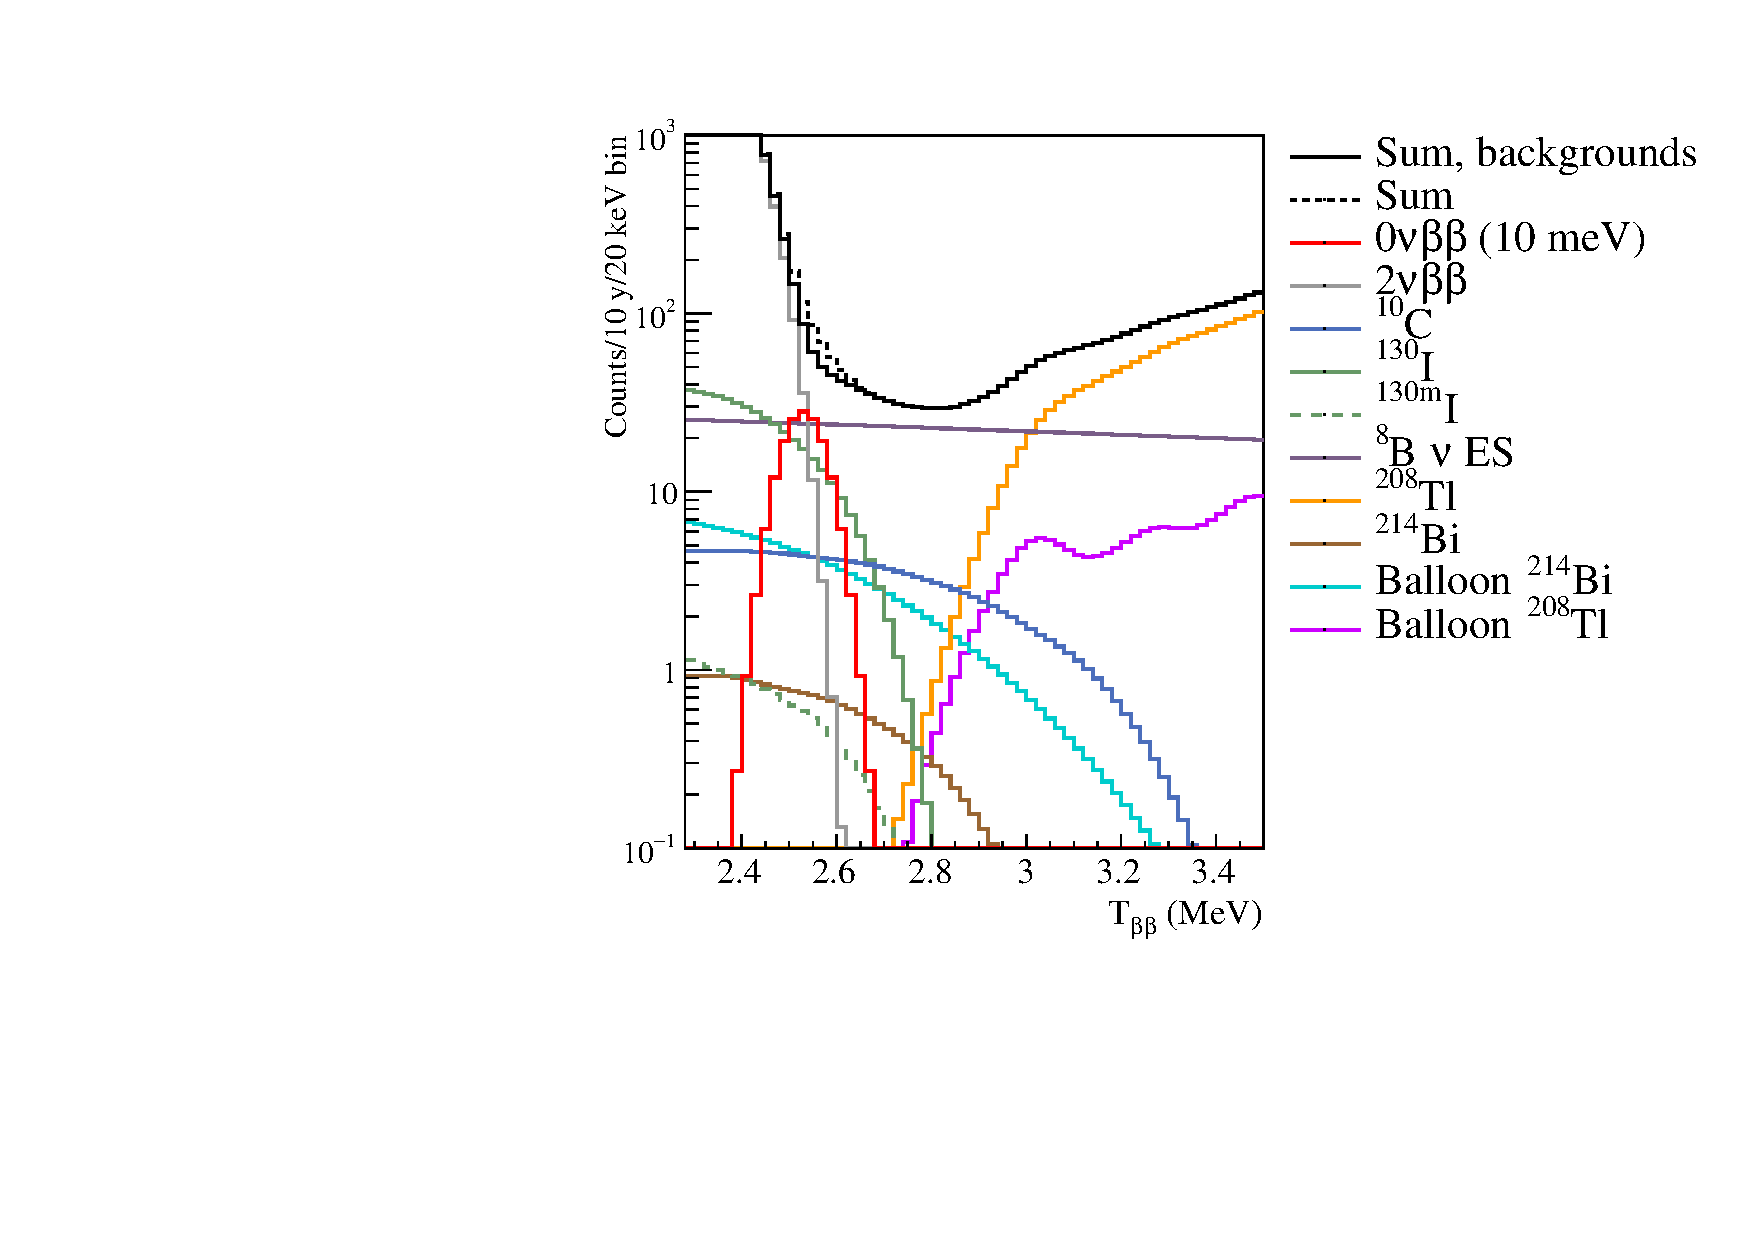
\includegraphics[width=\textwidth]{dbd/spectrum_plot_te_5.pdf}
 \caption{5\% $^{nat}$Te loading}
 \label{fig:spectrum-te}
\end{subfigure}
\begin{subfigure}[b]{0.45\textwidth}
 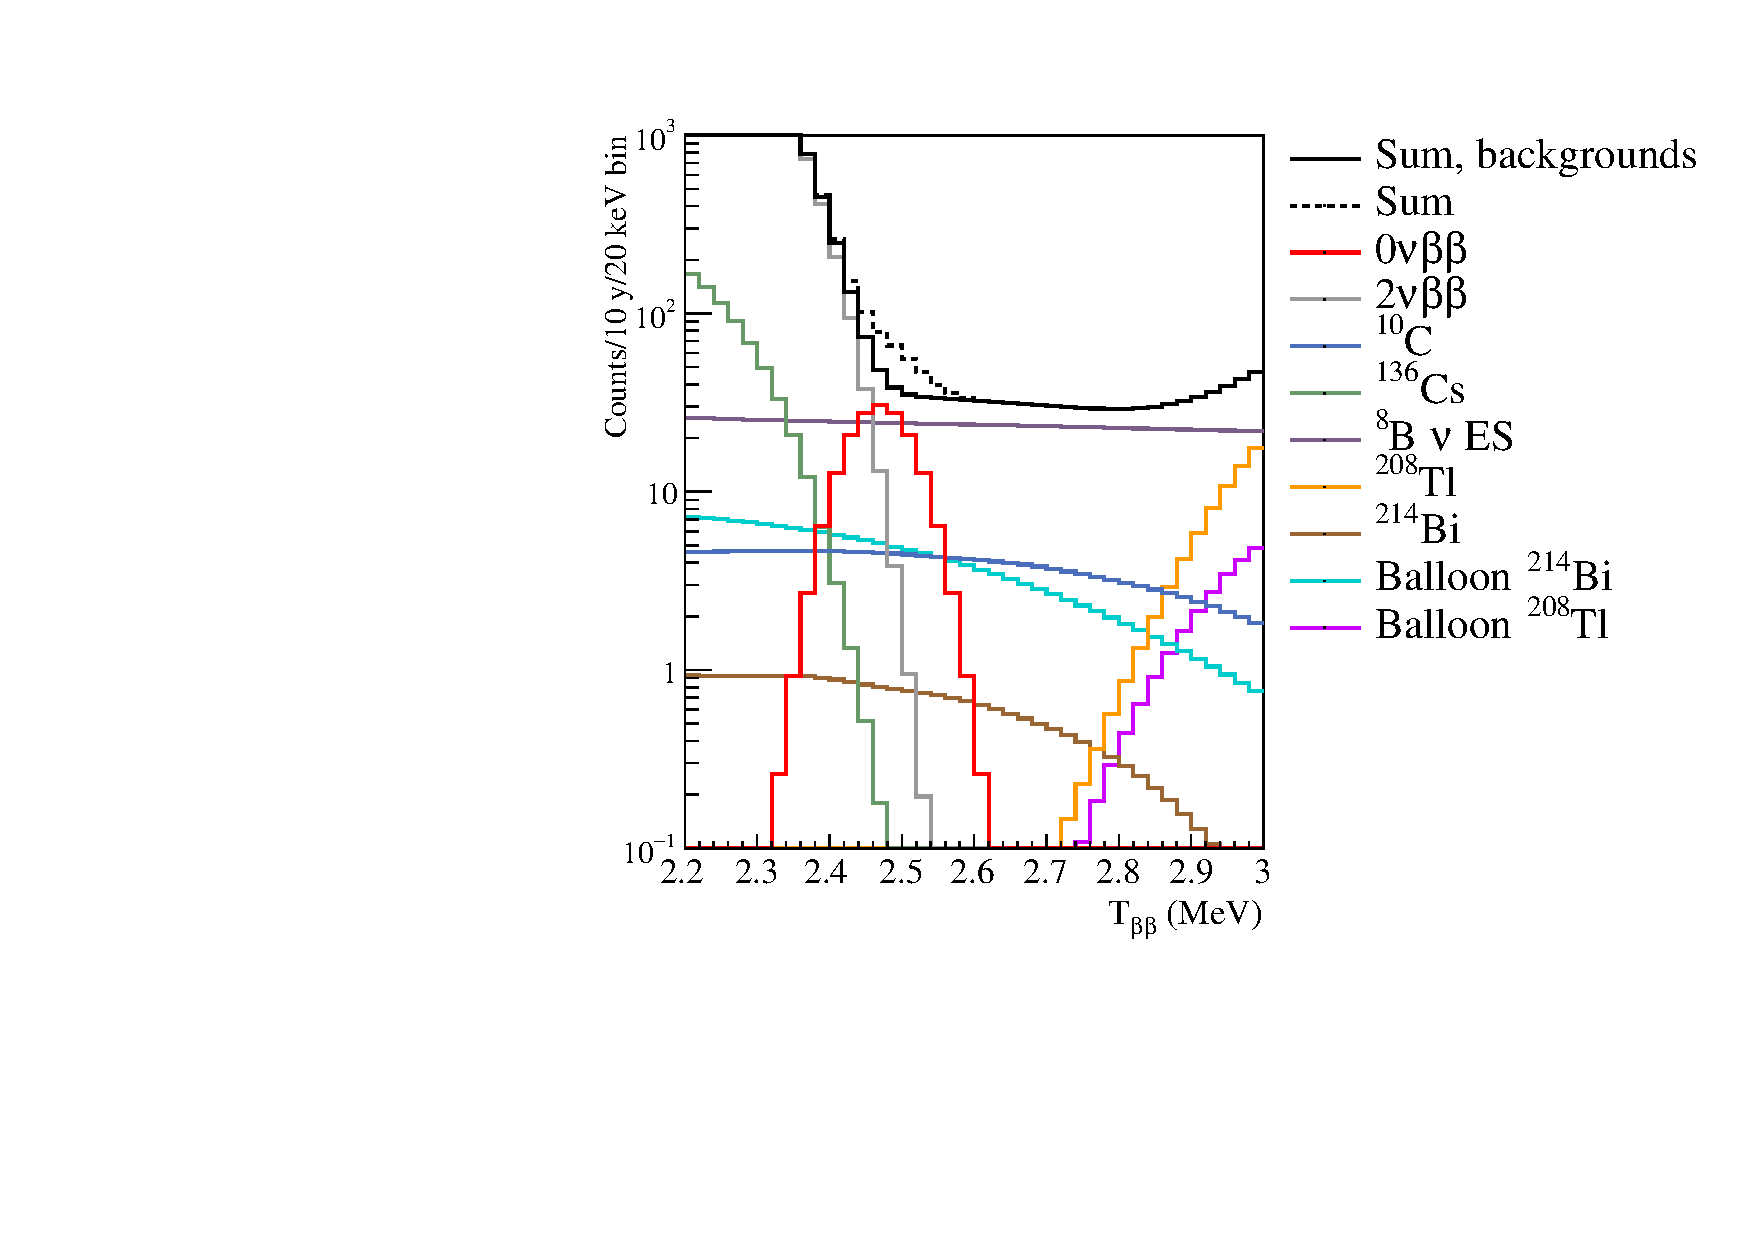
\includegraphics[width=\textwidth]{dbd/spectrum_plot_xe.pdf}
 \caption{3\% $^{enr}$Xe loading}
 \label{fig:spectrum-xe}
\end{subfigure}
\caption{Energy spectra near the NLDBD endpoint for events within the 7 m fiducial volume. A rejection factor of 92.5\% is assumed for $^{10}$C of , of 99.9\% for $^{214}$Bi, of 50\% for the balloon backgrounds, and 50\% for the $^8$B solar neutrinos.}
\label{fig:spectrum-plots}
\end{figure}

\noindent
%{\bf TODO:} Comment on prohibitive Xe costs?

\subsubsection{Alternative Isotopes}

Few alternative isotopes have been explored, which would be favorable in terms of annual abundance and costs: $^{100}$Mo, $^{82}$Se and $^{150}$Nd. For all these isotopes the main limiting factor is the leakage of the 2$\nu\beta\beta$ in the signal ROI, which highly increased due to the shorter half-life of the corresponding decay mode. A loading of 2\% for Se and Nd has been chosen based on results of stability tests in table-top experiments. For Mo a loading up to 3\% seems to maintain good stability and optical properties. In case of Nd and Mo an enrichment factor of 90\% is considered, while the enrichment option for Se is considered less promising due to the smaller G$_{0\nu} M^{2}_{0\nu}$ value, and the larger costs (although a larger world annual abundance than Xe is available). The scintillator purity is kept at 10$^{-17}$g/g for both U and Th for all the mixtures.\\ 
For a 90\% enriched $^{150}$Nd, the expected limit on the half-life is 5.1$\times 10^{27}$ years, with a limit on the effective Majorana neutrino mass (IBM-2) is 7.6\,meV. Similar values are obtained with a 3\%, 90\% enriched, $^{100}$Mo loading (T$_{1/2}$ = 9.5$\times 10^{27}$ and $m_{\beta\beta}$ = 7\,meV).

%\begin{table}
%\centering
%\scalebox{0.9}{
%\begin{tabular}{cccc}
%\toprule
%                          & \multicolumn{3}{c}{\bf Events/ROI$\cdot$10 y} \\
%{\bf Signal}              & $^{nat}$Se  & $^{nat}$Mo   & $^{enr}$Nd \\
%\midrule
%Loading fraction (\%) & 2 & 3 & 2 \\
%Isotope fraction (\%) & 8.73 & 9.82 & 90 \\
%Loaded isotope mass [t] & 3.2 & 5.4 & 33.2 \\
%$0\nu\beta\beta$ (10 meV) & 21.4       & 21.7 & 31.4      \\
%\midrule
%$2\nu\beta\beta$          & 117.3 &  325.6  & 2042     \\
%$^8$B Solar ES  (50\%)           & 136.2     & 135.6 & 132.9      \\
%$^{10}$C  (92.5\%)                & 9.91       & 8.49 & 0.28       \\
%$^{100}$Tc \cite{eijiri14, eijiri17}                 & ---       & 0.34 & ---        \\
%$^{82}$Br \cite{eijiri14, eijiri17}               & 0.21        & --- & ---        \\
%$^{150}$Pm \cite{eijiri14, eijiri17}               & ---        & --- & 0.145       \\
%$^{208}$Tl                & 158.4       & 198.7 & 563.4      \\
%$^{214}$Bi  (99.9\%)               & 0.18        & 0.09 & --- (*)        \\
%Balloon $^{214}$Bi  (50\%)       & 3.8       & 3.0 & 0.2       \\
%Balloon $^{208}$Tl  (50\%)      & 31.7       & 31.0 & 50.5       \\
%\midrule
%{\bf Total}               & 457.8      & 702.8 & 2789.9      \\ \hline \hline
%Expected T$_{1/2}$ ($\times10^{27}$ yr) & 2.2 & 2.4 & 5.1 \\
%Expected mass (meV) & 15.5 & 13.8 & 7.6 \\ \hline
%\bottomrule
%\end{tabular}}
%\caption{Expected background counts in 10 years of data taking in the ROI. In parenthesis is shown the reduction factor applied. (*) Assumed 10$^{-16}$ g/g in U. Limits on the effect Majorana neutrino mass are obtained for 90\% C.L. (FC approach) with phase space factors from \cite{2012PhRvC..85c4316K} and matrix elements from \cite{Barea:2013wb} (g$_{A}$=1.269).}
%\label{table::dbd::alternatives}
%\end{table}

%\begin{figure}
%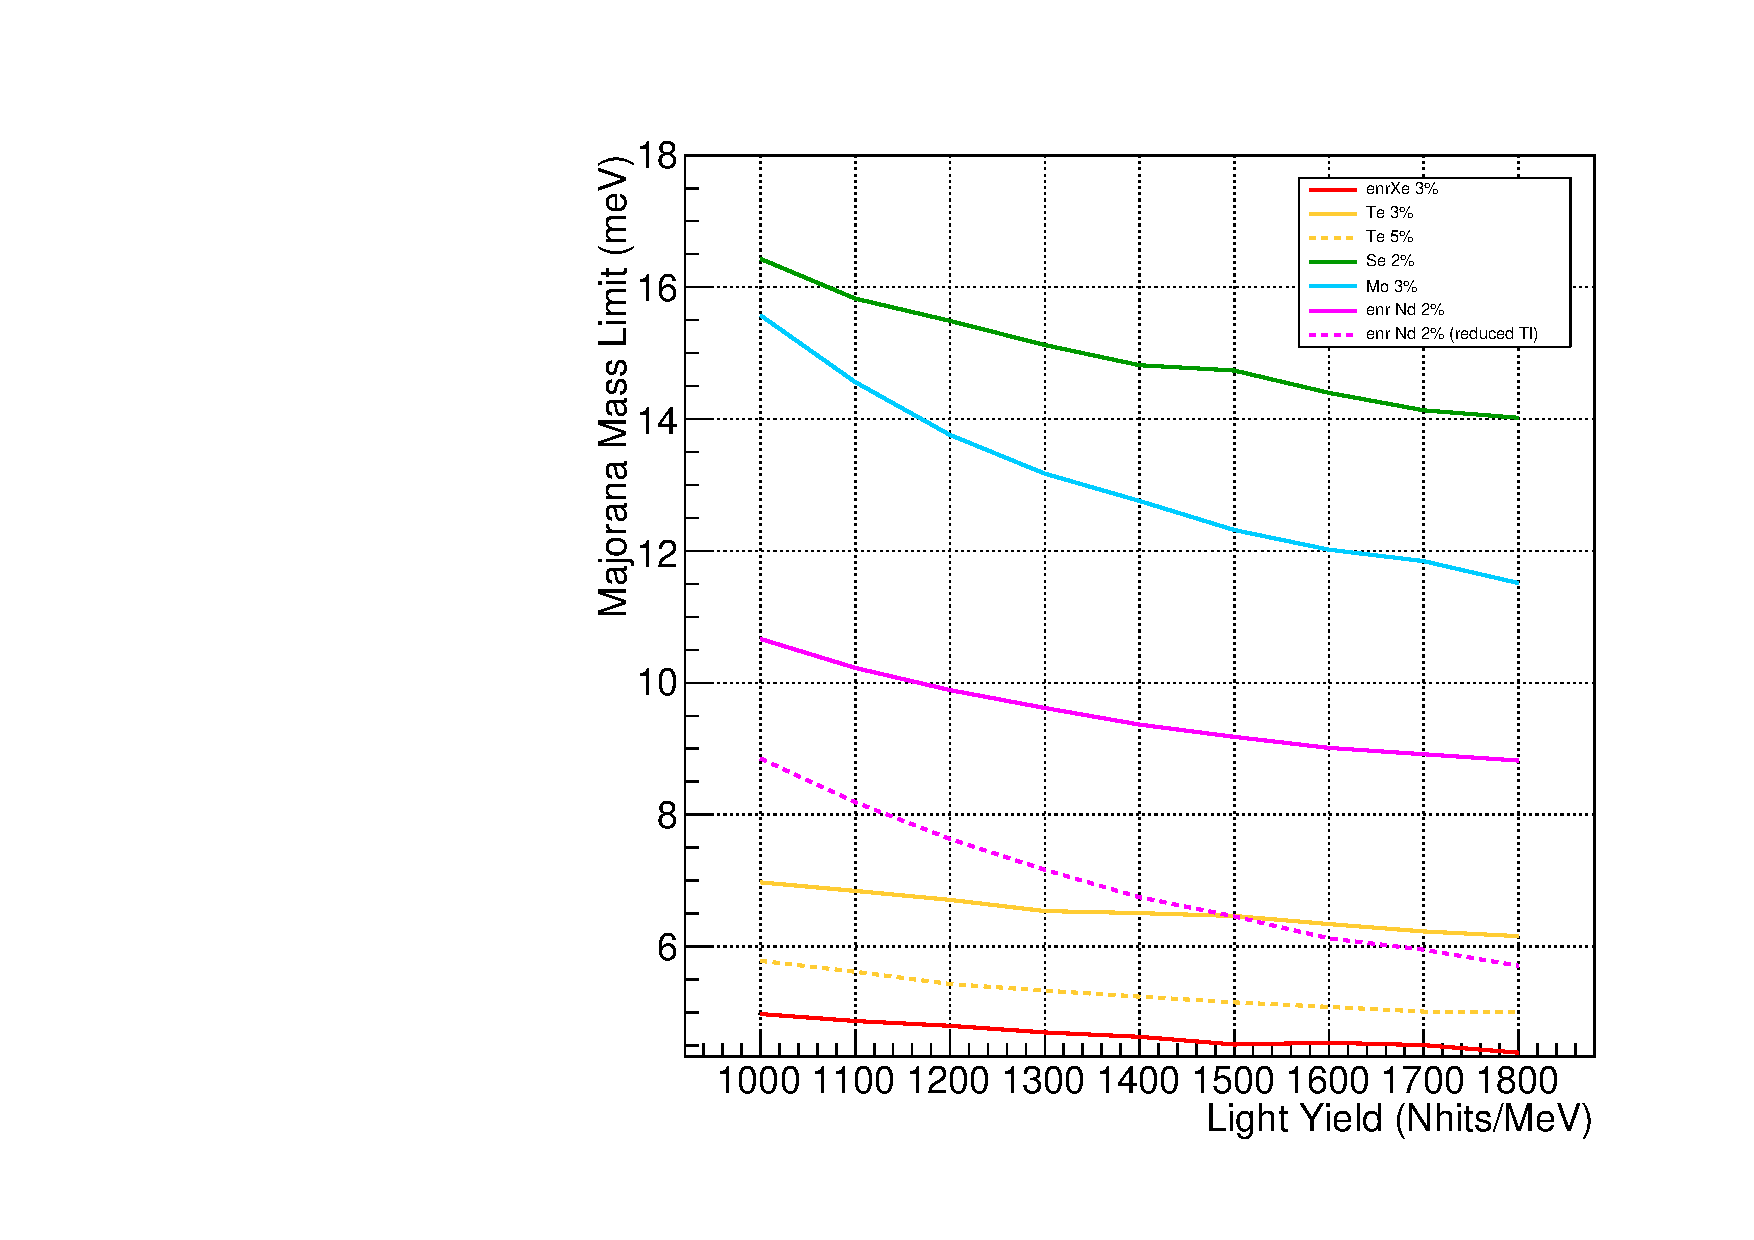
\includegraphics[scale=0.6]{dbd/ly_comparison_mass.pdf} 
%\caption{Comparison plot for various loading and isotopes. Shown is the limit on the effective Majorana neutrino mass as a function of the light yield.  3\%-$^{enr}$Xe loading still has the best limit, however 5\% Te and 2\%- $^{enr}$Nd are a competitive option. \label{fig::dbd::LY}}
%\end{figure}

%\section{Acknowledgements}
%
%\begin{thebibliography}{99}
%\bibitem{bxo16} N. Rossi, Neutrino 2016 Conference, London, 3---10 July 2016, \url{http://neutrino2016.iopconfs.org/IOP/media/uploaded/EVIOP/event_948/14.00__1_.pdf}
%\bibitem{mei09} D. M. Mei et al., Astropart. Phys. 31, 417–420 (2009).
%\bibitem{baudis15} L. Baudis et al., Eur. Phys. J. C 75, 485 (2015).
%\bibitem{zhang16} C. Zhang et al., Astropart. Phys. 84, 62--69 (2016).
%\bibitem{norm05} E. B. Norman et al., Nucl. Phys. B (Proc. Suppl.) 143, 508 (2005).
%\bibitem{bard97} D.W. Bardayan et al., Phys. Rev. C 55, 820 (1997).
%\bibitem{wang15} B.S. Wang et al., Phys. Rev. C 92, 024620 (2015).
%\bibitem{lozza15}  V. Lozza and J. Petzoldt, Astropart. Phys. 61, 62--71 (2015).
%\bibitem{snop16} S. Andringa et al., Advances in High Energy Physics 2016, 6194250 (2016).
%\bibitem{galb05} C. Galbiati, A. Pocar, D. Franco, A. Ianni, L. Cadonati, S. Schoenert, Phys.Rev. C 71 055805 (2005).
%\bibitem{gando16} Y Gando, Nuclear and Particle Physics Proceedings, vol. 273- 275, pp. 1842-1846 (2016).
%\bibitem{hagn00} T. Hagner et al., Astro. Phys. 14, 33--47, (2000).
%\bibitem{mei06} D. M. Mei and A. Hime, Phys. Rev. D 73, 053004 (2006).
%\bibitem{zbiri10} K. Zbiri, arxiv:0910.3714v3 [hep--ph] (2010).
%\bibitem{bxo2013} Borexino Collaboration, G. Bellini et al., JCAP08 49 (2013).
%\bibitem{SNO_3ph} SNO Collaboration, B. Aharmim et al., Physical Review C 88, 025501 (2013).
%\bibitem{Cuore017} C. Alduino et al., Eur. Phys. J. C 77 (2017).
%\bibitem{exo14}  J.B. Albert et al., Phys. Rev. C 89, 015502 (2014). 
%\bibitem{kam03} KamLAND Collaboration, K. Eguchi et al., Physical Review Letters 90, 021802, (2003).
%\bibitem{bxo09} Borexino Collaboration, C. Arpesella et al., Physical Review Letters 101,091302, (2008).
%\bibitem{gando13} A. Gando et al. Phys. Rev. Lett. 110, 062502 (2013).
%\bibitem{radiopurityorg} \url{https://www.radiopurity.org/rp/rp/_design/persephone/index.html?all}
%\bibitem{kamLAND_Zen} I. Shimizu, Frontiers of liquid Scintillator Technology (FroST16), March 18, 2016
%\url{https://indico.fnal.gov/getFile.py/access?contribId=45&sessionId=25&resId=0&materialId=slides&confId=10355}
%\bibitem{eijiri14} H. Ejiri and S. R. Elliott, Phys. Rev. C 89, 055501, (2014).
%\bibitem{eijiri17} H. Ejiri and S. R. Elliott, Phys. Rev. C 95, 055501 (2017).
%\bibitem{decay0} O.A.Ponkratenko, V.I.Tretyak, Yu.G.Zdesenko, Phys. At. Nucl. 63, 1282   (2000)  (nucl-ex/0104018)
%\bibitem{2012PhRvC..85c4316K} Kotila, J., \& Iachello, F. (2012). Phase-space factors for double-$\beta$ decay. Physical Review C - Nuclear Physics, 85(3), 034316. http://doi.org/10.1103/PhysRevC.85.034316
%\bibitem{Barea:2013wb} Barea, J., Kotila, J., \& Iachello, F. (2013). Nuclear matrix elements for double-$\beta$ decay. Physical Review C - Nuclear Physics, 87(1).
%\bibitem{KD-Zen} KamLAND-Zen Collaboration, Phys. Rev. Lett. 117, 082503 (2016).
%\bibitem{KZ-2011} Yoshihito Gando, Present Status of KamLAND-Zen, talk on International Workshop on Double Beta Decay and Neutrinos, Nov. 2011.
%\end{thebibliography}
%
%%\bibliographystyle{alpha}
%%\bibliography{sample}
%
%\end{document}


\subsection{Applied Antineutino Physics - S Dye for antinu group}
%\paragraph{Motivation}
%BRIEF intro to physics motivation, and status of the field: our major competitors
%\paragraph{XX with THEIA}
Electron antineutrinos stream freely from rapidly decaying fission products within nuclear reactors and from long-lived radioactive isotopes and their daughters within Earth \cite{agm15}. Important information about nuclear reactors, Earth, and the properties of neutrinos themselves comes from measuring the rate and energy spectrum of the interactions of these $1-10$ MeV antineutrinos. Detecting antineutrinos from nuclear reactors at short \cite{nucifer15,songs07} and long \cite{nudar13,snif10} distances monitors the operation and identifies the location and power of the reactor with applications for nuclear non-proliferation \cite{adam10}. Such detections also provide fundamental understanding of neutrinos \cite{reines53,reines76,jgl08}. Detecting antineutrinos from the nuclear cascades of thorium-232 and uranium-238 within Earth \cite{kl05} estimates terrestrial radiogenic heating \cite{gando13,agostini15}, leading to a more complete understanding of the composition, structure, and thermal evolution of our planet \cite{dye_etal15}. 

Global antineutrinos emerge from nuclear beta-minus decays, which produce a characteristic energy spectrum for each isotope. While the mixture of isotopes decaying within a source uniquely determines the energy spectrum of the emitted antineutrinos, neutrino oscillations distort the spectrum of detected antineutrinos in a pattern determined by the distance from the source. The rate and energy spectrum of global antineutrino interactions varies dramatically with surface location. The following discussion assumes a $50$-kT Theia with an energy-independent antineutrino detection efficiency of $90$\% located at SURF. Figure (theia_reac_geo.pdf) shows the detected energy spectrum of the predicted rate of antineutrinos from various sources.

Geo-neutrino observations probe the quantities and distributions of terrestrial heat-producing elements uranium and thorium. The quantities of these elements gauge global radiogenic power, offering insights into the origin and thermal history of the Earth. Spatial distributions reveal the initial partitioning and subsequent transport of these trace elements between metallic core, silicate mantle, and crust types. Ongoing observations at underground sites in Japan and Italy record the energies but not the directions of geo-neutrinos from uranium and thorium. Without directions pointing back to source regions, disentangling the signals from various reservoirs requires resolution of differing rates or energy spectra at separate sites. Due to limited statistics and perhaps insufficient site contrast, the observations at Japan and Italy do not yet measure distinct rates or energy spectra. The large exposure possible with Theia offers an opportunity to remedy this situation.

Geo-neutrino events per year $1318$ ($1031$ U and $287$ Th), which is $43.9 \pm 1.2$ TNU assuming statistical error only. This corresponds to a flux of $4.90 \pm 0.13 \times 10^6$ cm$^{-2}$ s$^{-1}$, assuming Th/U $=3.9$. For comparison, the latest reported geo-neutrino rates from KamLAND and Borexino correspond to $3.4 \pm 0.8 \times 10^6$ cm$^{-2}$ s$^{-1}$ and $5.0 \pm 1.3 \times 10^6$ cm$^{-2}$ s$^{-1}$, respectively. While consistent with the Borexino measurement, the predicted Theia measurement is almost $2 \sigma$ greater than the KamLAND measurement after just one year of livetime. This would provide the first evidence for surface variation of the geo-neutrino flux.


Reactor antineutrino events per year $985$.

\it THIS IS IT FOT THIS WEEK. MORE COMING SOON.

%What we bring to the table - pros of THEIA design \newline
%Sensitivity estimates with baseline design (one of THEIA i--iii)
%\paragraph{Detector Requirements}
%A summary of the impact of different detector choices i.e. what happens if we stray from the relevant baseline


\subsection{Sterile Neutrinos - \bf volunteers?}
\paragraph{Motivation}
BRIEF intro to physics motivation, and status of the field: our major competitors
\paragraph{XX with THEIA}
What we bring to the table - pros of THEIA design \newline
Sensitivity estimates with baseline design (one of THEIA i--iii)
\paragraph{Detector Requirements}
A summary of the impact of different detector choices i.e. what happens if we stray from the relevant baseline


%\subsection{Astrophysical Sources}
%\subsubsection{Detector Simulation}
%Summary of simulation used in following sections, including e.g. high energy physics list, specific parameters for each detector configuration.

\subsubsection{Solar Neutrinos - GDOG, R Bonventre}
\paragraph{Motivation}
BRIEF intro to physics motivation, and status of the field: our major competitors
\paragraph{XX with THEIA}
What we bring to the table - pros of THEIA design \newline
Sensitivity estimates with baseline design (one of THEIA i--iii)
\paragraph{Detector Requirements}
A summary of the impact of different detector choices i.e. what happens if we stray from the relevant baseline


\subsubsection{Supernova Neutrinos}

\paragraph{Motivation}

The neutrino burst detected from the next galactic Supernova will provide us with a wealth of information on the dynamics of the core collapse (neutronization, reheating, proto-neutron star cooling) and the properties of the neutrinos themselves (mass hierarchy, absolute mass scale, collective oscillations). Since the first detection of Supernova neutrinos in 1987, the scientific community has not become tired to predict new effects and their signatures that are potentially to be extracted from the neutrino signal. So while we are uncertain what to expect from the next event and how different effects will overlay, it is beyond doubt that only a concerted effort making use of the complementary strengths of all the neutrino observatories available will enable us to extract the full amount of information. Moreover, this combined analysis has to reach beyond neutrino detectors, including gravitational wave and (if present) optical signatures to appreciate the full picture.

If a Supernova neutrino burst would pass by the Earth today, hundreds of events would be expected in several smaller observatories (LVD, Borexino, KamLAND, SNO+, HALO to name but a few). However, the largest event statistics would be collected by the two large Cherenkov detectors, Super-Kamiokande (SK) and IceCube. Ten years from now, we may expect that two further players will appear on the stage: JUNO offering a liquid scintillator target, and DUNE allowing SN neutrino detection in liquid argon. In the most simplified picture, SK, JUNO and IceCube will dominate the information on $\bar\nu_e$ flux and energies, while DUNE has the potential for a high-statistics $\nu_e$ measurement. JUNO will provide information on the combined flux of $\nu_\mu$ and $\nu_\tau$ and antineutrinos (in the following, we use the conventional denotation $\nu_x$).

\paragraph{Impact of THEIA} In the following, we assume the THEIA-ii detector configuration, i.e.~a 50\,kt neutrino target filled with a WbLS containing 10\,\% of organic scintillator. With 90\,\% optical coverage, the expected photoelectron yield for a 10\,\%-WbLS is $\sim$200\,p.e./MeV (75\,\% scintillation), providing a stochastic energy resolution of 7\,\%. Thus, THEIA will provide a threshold in the low MeV range and $-$ given the high coverage $-$ spectroscopic capabilities close to that of current-day organic liquid scintillator detectors. Importantly, THEIA will provide a clear neutron tag, allowing to discriminate Inverse Beta Decay (IBD) events from other single-event backgrounds.
\medskip\\
Given this additional features, what can THEIA add to the global picture of SN neutrino observations? 
\begin{itemize}
\item a high-statistics IBD ($\bar\nu_e$) signal, offering considerably better energy resolution than SK and about twice its statistics; both will prove very useful when trying to correlate spectral features changing over time with other signals, e.g.~gravitational wave emission during the SASI phase, or when looking for energy-dependent oscillation patterns (e.g.~the spectral swaps induced by collective oscillations)
\item improved pointing accuracy for the $\nu_e$ elastic scattering signal, improving the current day $\sim$3$^\circ$ resolution of SK to the level of 1$^\circ$ or better. The key is the almost complete event-by-event subtraction of IBD events enabled by the neutron capture tag \cite{Tomas:2003xn}; SK+Gd can expect a similar improvement but offers a neutron tagging efficiency of only $\sim$70\,\%
\item the chance to glimpse the initial $\nu_e$ neutronization burst \cite{Kachelriess:2004ds}: however, as $\cal O$(10) events are expected for a SN at 10\,kpc, detailed information can only be expected for a relatively nearby Supernova
\item relative to SK and JUNO, a $\bar\nu_e$ detector on the other side of the Earth, allowing to study Earth matter effects in $\bar\nu_e$ in a direct spectral comparison; note that, again, energy resolution is a key parameter here.
\end{itemize}

\paragraph{Spectroscopy of SN neutrinos in THEIA}

Compared to all other running and upcoming detectors (except Hyper-Kamiokande), 50\,kt of WbLS will constitute the largest neutrino target, roughly doubling the available statistics of IBDs in water (SK) and scintillator (JUNO) detectors. Moreover, THEIA will provide both good energy and directional resolution, offering handles to discriminate between different neutrino reaction channels.

As stated above, present knowledge of the SN neutrino emission and neutrino properties does not allow for a precise prediction of the expected signal. Nevertheless, to provide a scale of the expected signal we list in table \ref{tab:snrates} the time-integrated event rates for a Supernova in 10\,kpc distance (close to the galactic center), using energies and fluxes predicted by the GVKM (Gava-Kneller-Volpe-McLaughlin) model \cite{Gava:2009pj} and the cross-sections provided by the SNOwGLoBES framework.

\begin{table}[h!]
\centering
\begin{tabular}{lclr}
\hline
Channel & & Reaction & Event rate \\
\hline
Inverse Beta Decay & (IBD) & $\bar\nu_e+p\to n+e^+$ & 9,900 \\
 Electron Scattering & (ES) &$\nu+e \to e+\nu$ & 480 \\
 CC on $^{16}$O & ($\bar\nu_e$O) & $\nu_e+ {^{16}{\rm O}} \to  {^{16}{\rm F}}+e^-$ & 170 \\
 & ($\nu_e$O) & $\bar\nu_e+ {^{16}{\rm O}} \to  {^{16}{\rm N}}+e^+$ & 220 \\
NC on $^{16}$O & (NC) &  $\nu + {^{16}{\rm O}} \to  {^{16}{\rm O}^*}+\nu$ & 550 \\
\hline
\end{tabular}
\caption{Neutrino event rates expected in 50\,kt of WbLS (10\,\% scintillator) for a core-collapse Supernova at 10\,kpc distance. Neutrino spectra and fluxes follow the GVKM model \cite{Gava:2009pj}.}
\label{tab:snrates}
\end{table}

\noindent {\bf Event rates.} The signal is vastly dominated by the $\bar\nu_e$-induced IBD events, followed by the NC reactions of all neutrino flavors on oxygen and elastic scattering off electrons. Note that as WbLS contains as well carbohydrates, THEIA will detect relevant numbers of neutrino events on carbon: For a 10\,\% WbLS, $\sim$250 events from NC carbon reactions are expected, inducing a gamma peak at 15\,MeV (not shown in fig.~\ref{fig:snspectra}), adding to the information on the integrated neutrino flux.
\medskip\\
{\bf Energy spectrum} Given its large target mass and good energy resolution, THEIA will offer detailed spectral information for the $\bar\nu_e$ flux (based on IBD events). Moreover, less precise but still relevant spectral data will be available for all other neutrino flavors that are detected in their hundreds. In figure \ref{fig:snspectra}, we show the expected event spectra as a function of their visible energy, already smeared with a 7\,\% energy resolution. As for the rate, the IBD signal dominates the interaction rates for all energies, with the noteworthy exception of the two low-energy $\gamma$ lines from the NC reaction on oxygen. However, differently from current-day water Cherenkov detectors, the neutron tag for IBD events allows to subtract the IBD signal on an event-by-event basis, providing better access for a separate study of the subdominant reaction channels. As a consequence, the gamma lines from the NC reaction are easy to extract from the remaining spectrum, providing a flavor-independent measurement of the neutrino flux \cite{Langanke:1995he,Haxton:1987kc}. Moreover, the presence of scintillation light and high energy resolution enables separate detection of the strongest gamma lines and thus a measurement of their relative spectral contributions. In case of a very efficient IBD subtraction (close to 100\,\% efficiency), there will be even some potential to separate the remaining ES, $\nu_e$O and $\bar\nu_e$O channels: ES events are strongly correlated with the SN direction and will stand out in any case (see below). Moreover, the re-decay of $^{16}$N potentially offers a delayed coincidence signature for $\bar\nu_e$O events: The remaining $\nu_e$O would then provide access to a small but pure sample of electron neutrino events. 
\begin{figure}[h!]
\centering
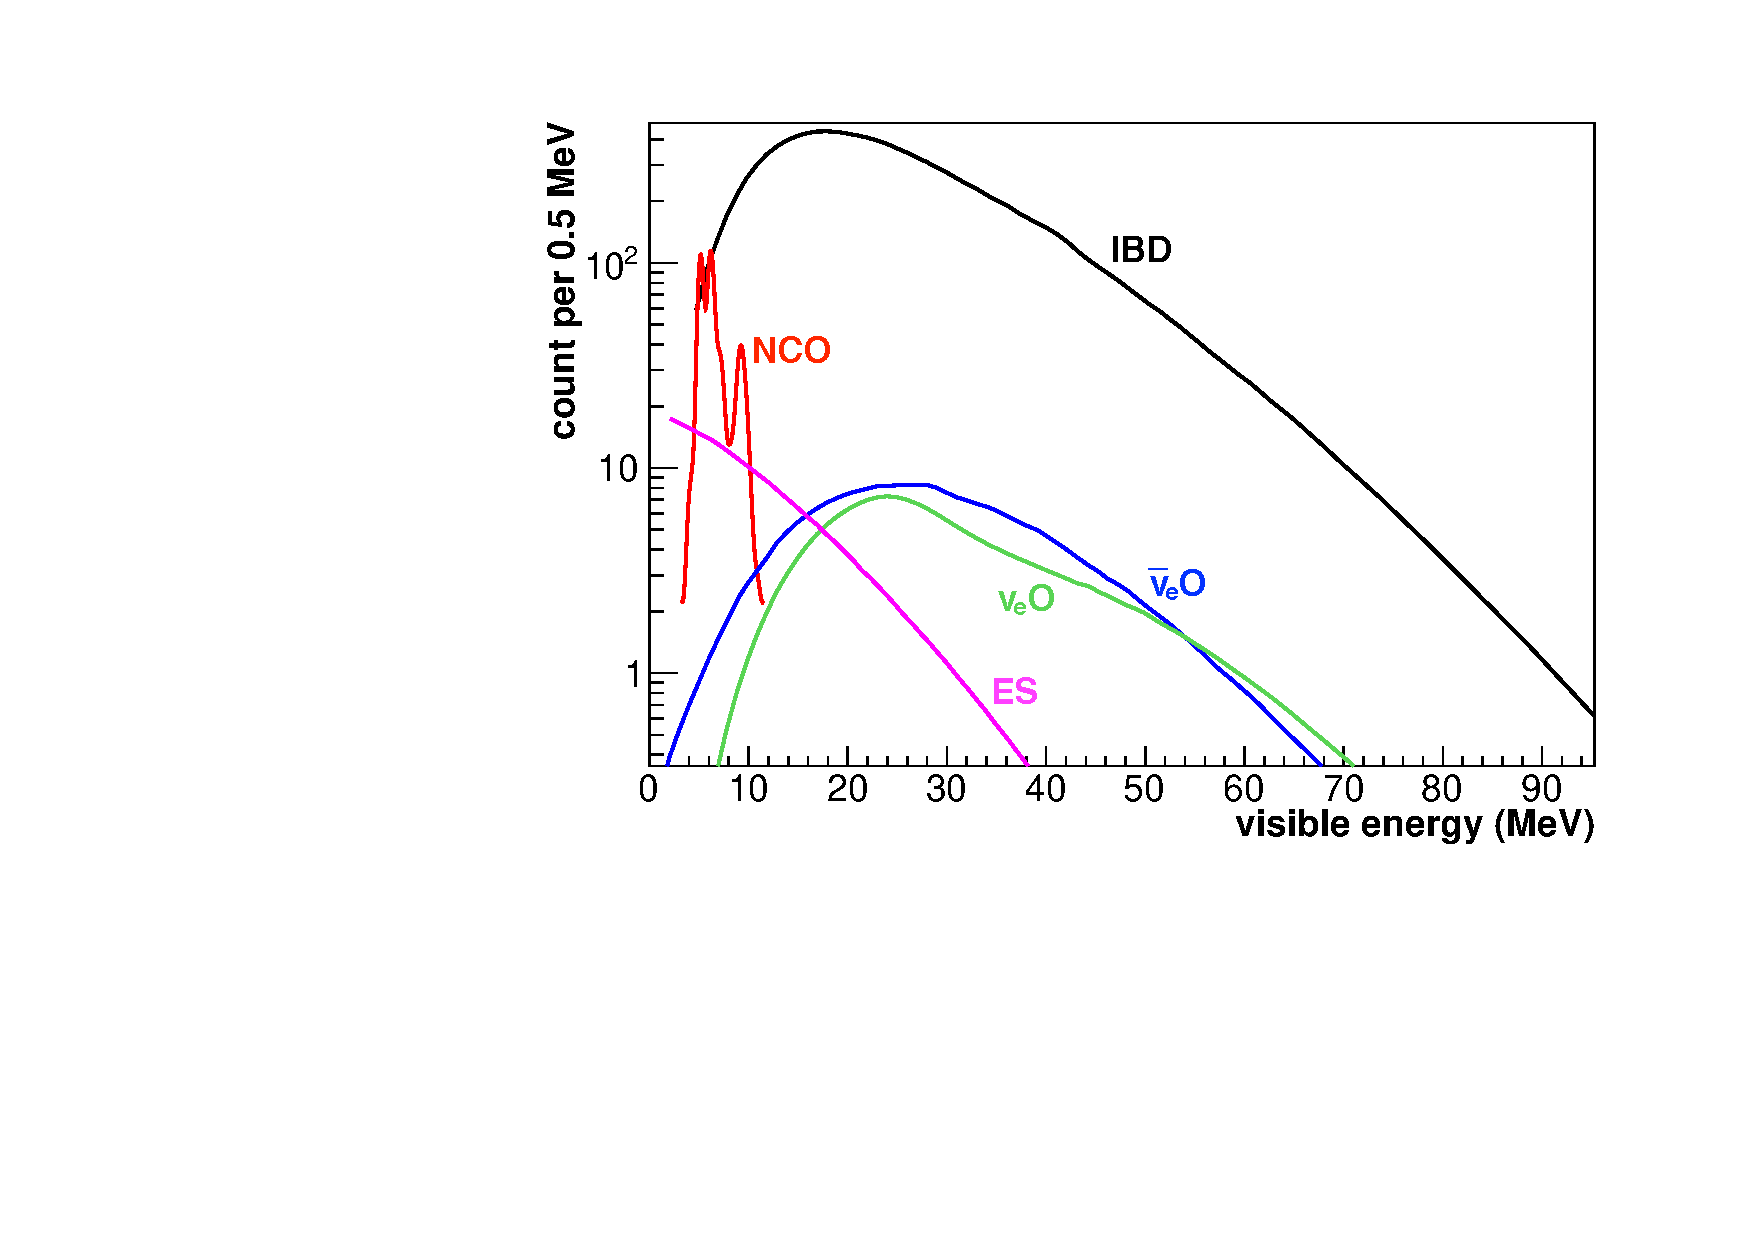
\includegraphics[width=0.67\textwidth]{pics/sn_spectra.pdf}
\caption{Visible energy spectra for prompt events expected in 50\,kt of WbLS, assuming a Gaussian energy resolution of 7\,\% at 1\,MeV. Neutrino spectra and fluxes follow the GVKM model \cite{Gava:2009pj}.}
\label{fig:snspectra}
\end{figure}
\medskip\\
\noindent{\bf Time-dependent features} A time-dependent measurement of the neutrino signal is especially interesting for studying the different phases and physical processes underlying the core collapse. For a Supernova in 10\,kpc distance, the initial neutronization burst will translate only to a small number of ES and $\nu_e$O events in THEIA, $\cal O$(10). However, if the SN were to happen closer and if the information of several detectors (especially DUNE) is combined, energy, flux and flavor content may be studied in detail. On its own, THEIA will provide detailed spectral information of the $\bar\nu_e$ flux during the accretion phase, nicely complementing the flux information available from IceCube. 
\medskip\\
{\bf SN neutrino pointing.} In Water Cherenkov Detectors like SK, the direction of the incoming neutrino burst can be determined based on the recoil electrons from ES: Given the relatively large neutrino energies, the electrons are very tightly aligned with the initial momentum of the neutrino. In SK, this will be sufficient to pinpoint the location of the SN within 3-4 degrees \cite{Abe:2016waf}. The most important factor limiting resolution in this case is the relatively high background formed by the only slightly directional positrons from IBD interactions. In the angular distribution of events, a peak consisting of $\sim10^2$ ES events has to be found over a flat background of several thousand IBDs.

It has been suggested (e.g.~in \cite{Tomas:2003xn}) that the directional resolution can be considerably enhanced if the IBD events can be discriminated based on the delayed neutron tag, reducing the flat background. This represents one of the key features of SN neutrino detection in THEIA: As an example, the left panel in figure~\ref{fig:snpointing} shows the angular distribution for an SN neutrino burst (Wilson model \cite{Totani:1997vj}, 10\,kpc distance), where an efficiency of 90\,\% is assumed for IBD rejection: While the ES events are clearly peaked in the direction of the SN ($\Delta\theta=\Delta\phi=0^\circ$), the reduced IBD background constitutes only a minor background noise. 

We studied the effect of IBD background reduction on the directional resolution based on a toy MC of the signal. For this, we fitted the output angular distribution with a radial exponential plus flat background resolution, regarding three different cases: No, 90\,\% and full IBD reduction with full detection efficiency for ES events. For the latter, we considered full event kinematics (linking electron and neutrino momentum directions) and an intrinsic angular resolution of 10$^\circ$. The results are depicted in the right panel of figure~\ref{fig:snpointing}, once for a fiducial mass of 45\,kt in the THEIA-ii configuration where close to full detection efficiency for the delayed neutron tag can be assumed, and once for half this  mass to allow for an easier comparison to current SK pointing capabilities. While we can reproduce the $\cal O$(3-4$^\circ$) pointing accuracy of SK, THEIA will reach an angular resolution of close to 1$^{\circ}$.

It should be noted that SK+Gd will feature as well improved pointing precision based on the available delayed neutron tag. For this case, angular resolution can be estimated to $\sim$2$^{\circ}$.
\begin{figure}[h!]
\centering
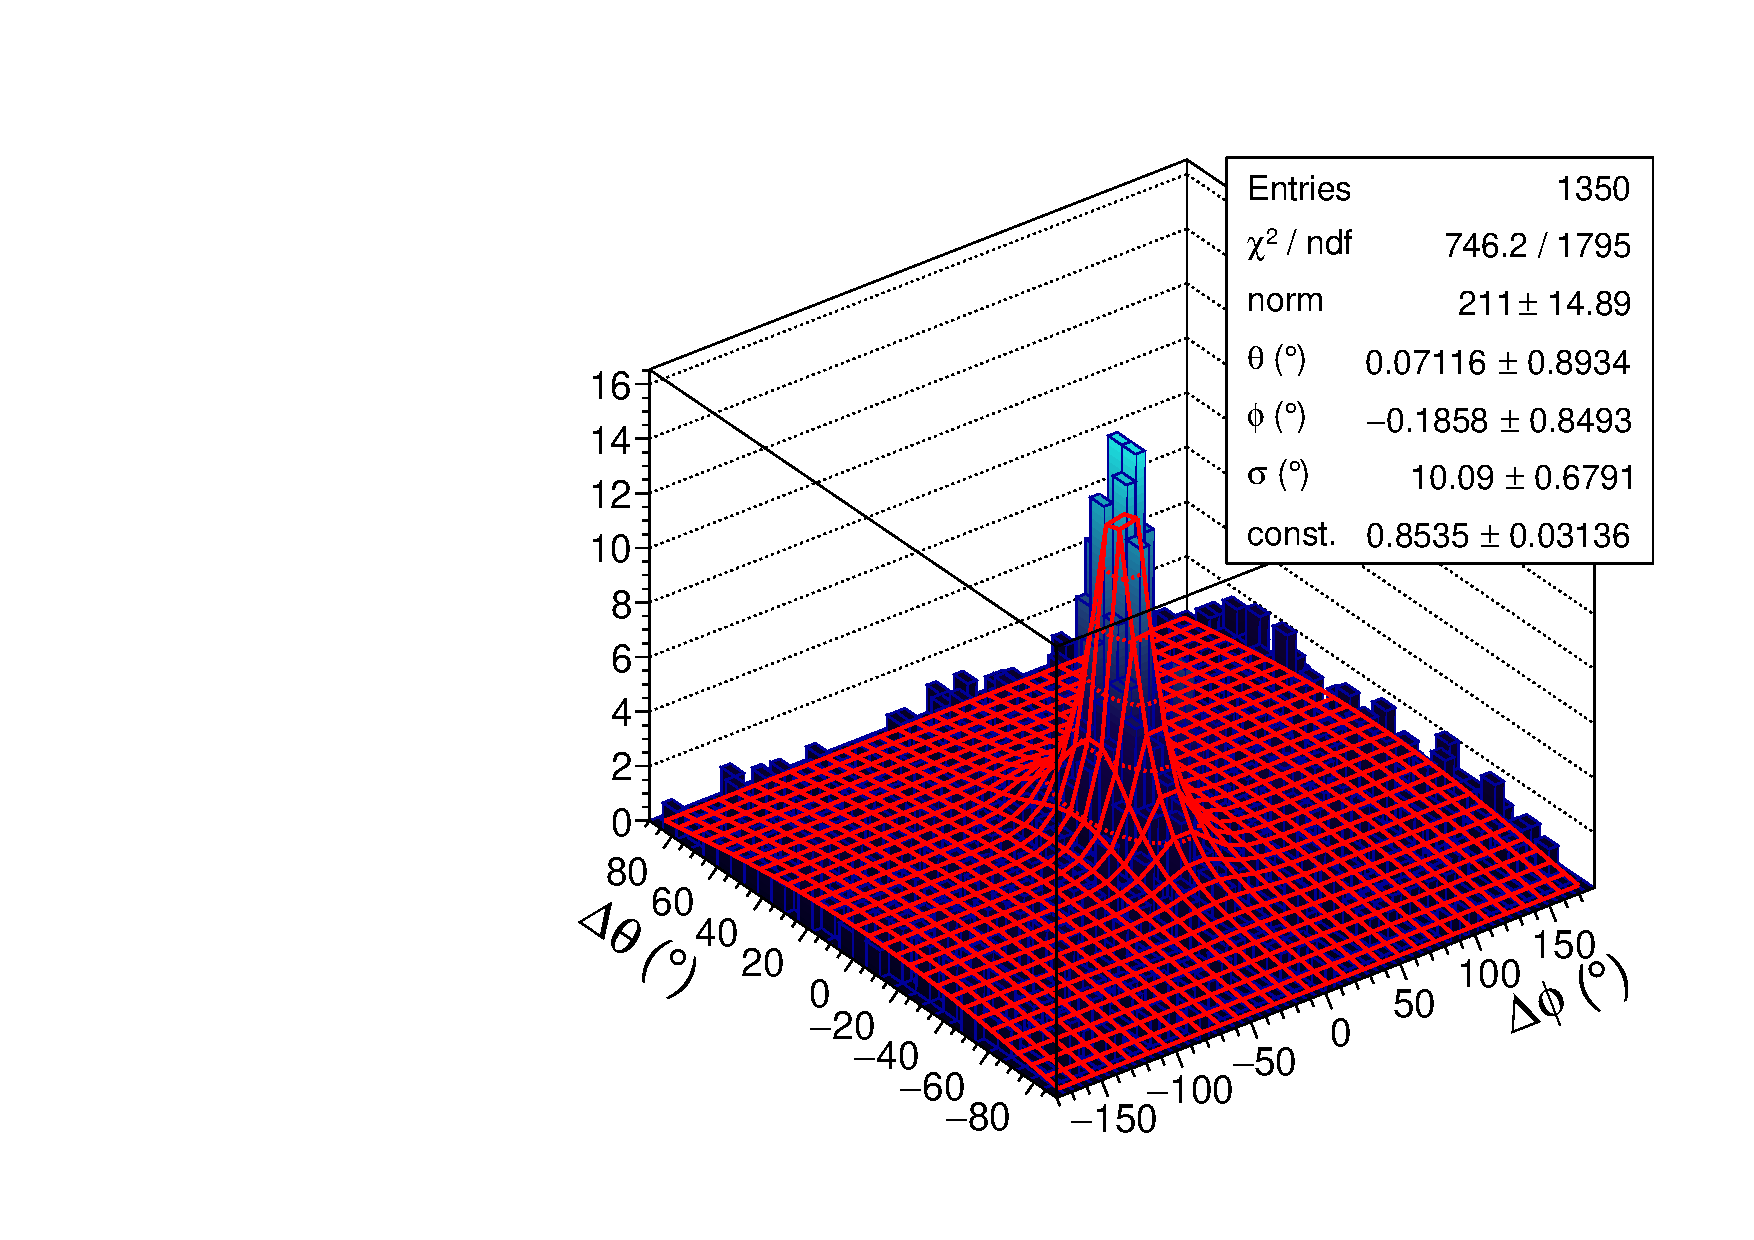
\includegraphics[width=0.5\textwidth]{pics/sn_directionality_fit.pdf}
\hfill
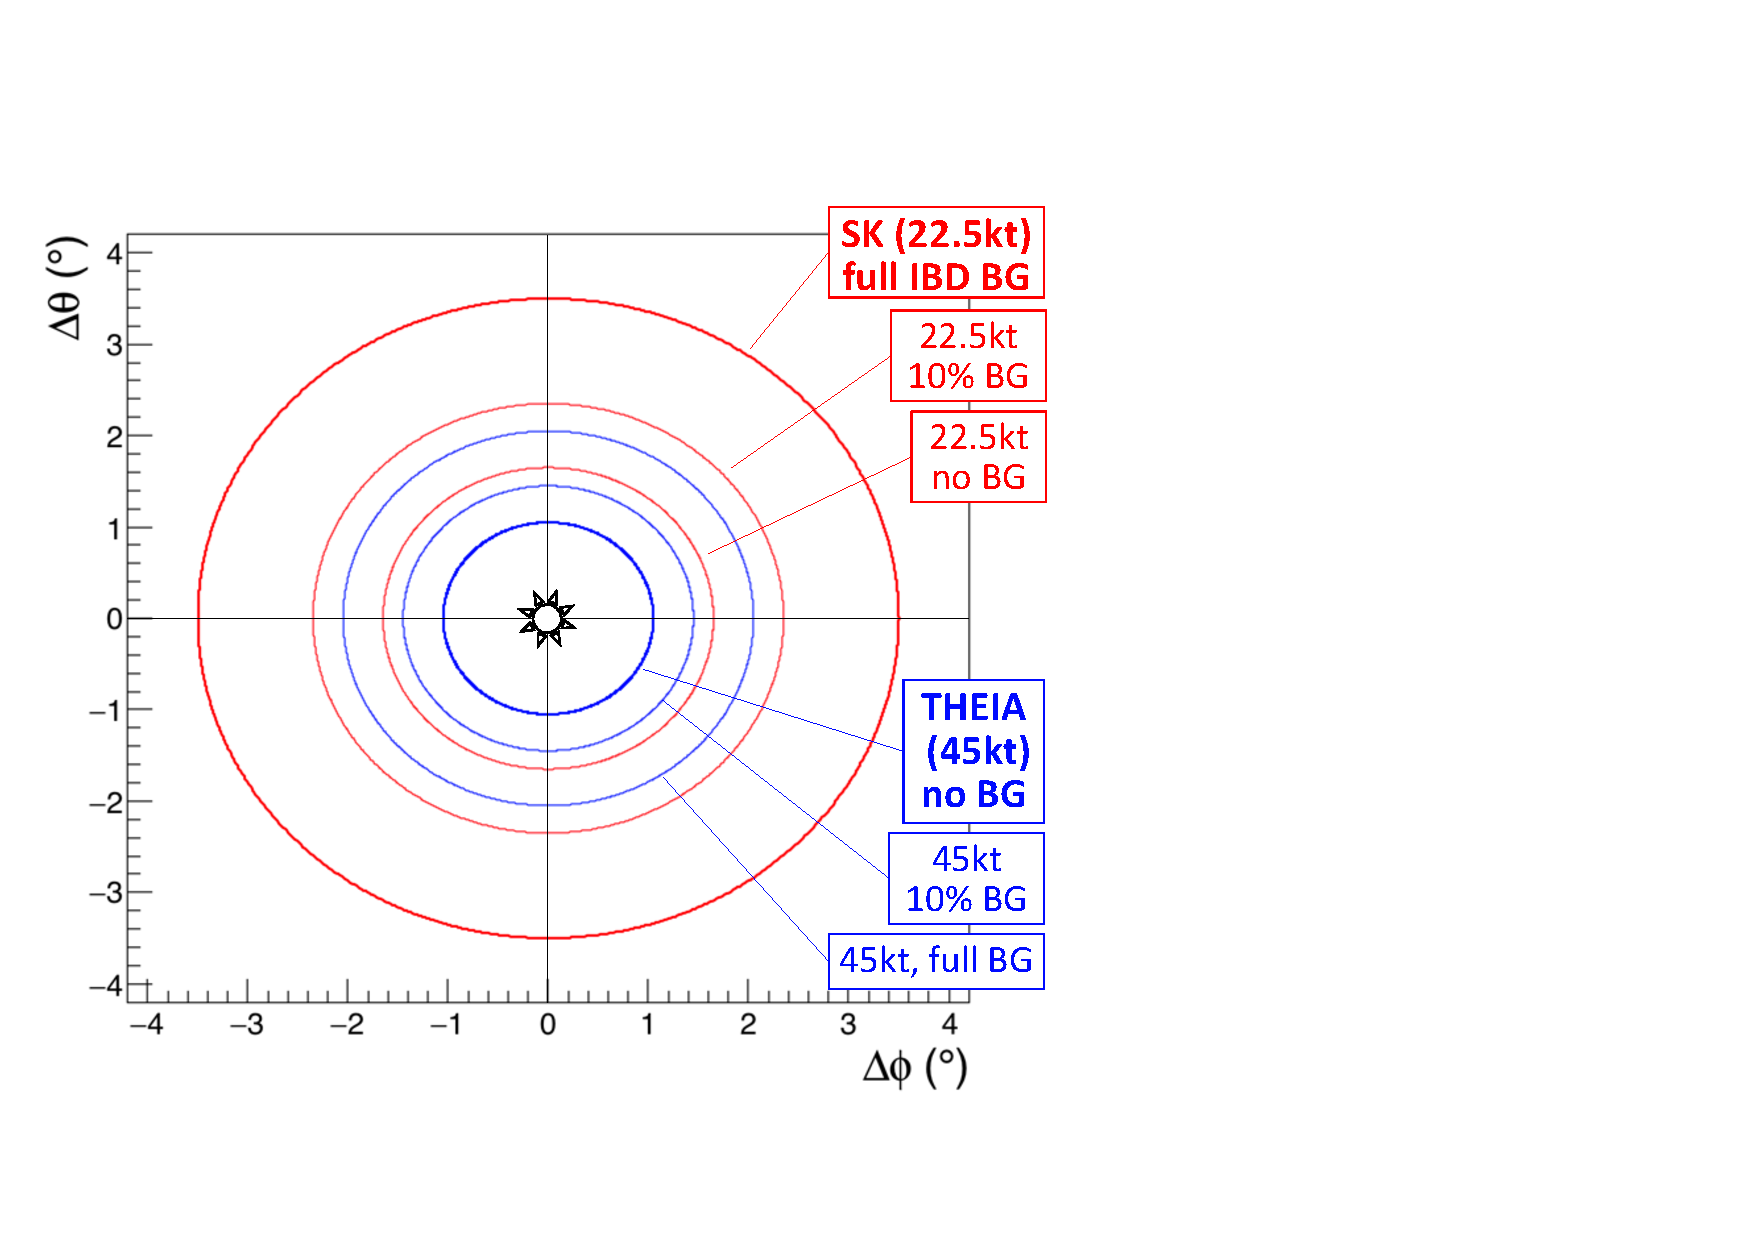
\includegraphics[width=0.46\textwidth]{pics/sn_position_resolution.pdf}
\caption{SN pointing capability of THEIA, based on the reconstruction of the ES directional signal. {\it Left panel:} Example angular distribution, assuming 90\,\% in the flat IBD spectrum. Based on a fit to this and similar distributions (red net), the {\it right panel} depicts the pointing accuracy for THEIA, assuming different IBD background levels for 45\,kt as well as 22.5\,kt target mass.}
\label{fig:snpointing}
\end{figure}

\subsubsection{Diffuse Supernova Neutrino Background - S Dye for antinu group}
\paragraph{Motivation}
BRIEF intro to physics motivation, and status of the field: our major competitors
\paragraph{XX with THEIA}
What we bring to the table - pros of THEIA design \newline
Sensitivity estimates with baseline design (one of THEIA i--iii)
\paragraph{Detector Requirements}
A summary of the impact of different detector choices i.e. what happens if we stray from the relevant baseline


\subsection{Indirect Dark Matter ?? }
From Michi -- there is still some interest in detecting decay/annihilation neutrinos in the multi-MeV range where THEIA would probably be able to place very competitive limits (as I noticed speaking to a theorist from Brussels a few weeks ago). It would be an addition to the antineutrino WG. Certainly, it?s rather low priority, but we could put it there as a place-holder.
%\paragraph{Motivation}
%BRIEF intro to physics motivation, and status of the field: our major competitors
%\paragraph{XX with THEIA}
%What we bring to the table - pros of THEIA design \newline
%Sensitivity estimates with baseline design (one of THEIA i--iii)
%\paragraph{Detector Requirements}
%A summary of the impact of different detector choices i.e. what happens if we stray from the relevant baseline




%\section{Site Selection}
%
%Do we want to add this, or not really?  Maybe for the White Paper we should simply assume SURF?
%
%GDOG suggests to remove this section
%
%%\section{Baseline Detector Design}
%%\subsection{Detector Configuration Requirements}
%%Size, Depth, light yield, separation requirements
%%\subsection{WbLS Target}
%%\subsection{Photon Sensor Selection - Hybrid Scheme}
%
%\section{THEIA Timeline}
%
%Do we want to include anything on this?  Or does it simply risk that we are immediately out of date?
%
%GDOG suggests to remove this section


\section{Conclusions}

\textsc{Theia} offers a broad program of compelling science, covering topics in nuclear physics, high-energy physics, astrophysics, and geophysics.  These include: solar neutrinos and neutrinoless double beta decay; proton decay and long-baseline physics; supernova neutrinos and DSNB;  and geoneutrinos, respectively.

Use of the novel, potentially inexpensive WbLS target  allows construction of a precision detector on a massive scale.  
Successful identification of Cherenkov light in a scintillating detector would result in unprecedented background-rejection capability and signal detection efficiency via directionality and sub-Cherenkov threshold particle identification.  This low-threshold, directional detector could achieve a fantastically broad physics program, combining conventional neutrino physics with rare-event searches in a single, large-scale detector.
The flexibility of the WbLS target, of the options for isotope loading, and even of the detector configuration is a crucial aspect of \textsc{Theia}'s design.  As the field evolves, \textsc{Theia} has the unique ability to adapt to new directions in the scientific program, making it a powerful instrument of discovery that could transform the next-generation of experiments.  

The feasibility of a low energy solar neutrino measurement with a large WbLS detector depends on the backgrounds and angular resolution achievable. At currently measured levels, the limiting background appears to be \isotope[40]{K} in water.  Remaining backgrounds in water have little effect if they are kept to 1000 to 10000 times the level achieved in scintillator. The \isotope[11]{C} background has a small effect, which suggests that the overburden does not matter for this measurement. The impact of changes in scintillator and PMT coverage on energy resolution have relatively small effects,  suggesting that even at 0.5\% scintillator fraction, energy resolution is no longer the critical parameter to optimize. Instead, the impact of these changes on threshold and angular resolution will be the deciding factor.  With a baseline detector of 50-kT total volume (50\% fiducial), 90\% PMT coverage and a 5\% WbLS target, assuming  a $25^\circ$ angular resolution, a precision of several percent is possible for both CNO and pep neutrino fluxes.

Further studies hinge on additional R\&D, including the Cherenkov detection efficiency enhancement provided by deployment of fast photon sensors, and demonstration of quenching and particle ID capabilities in WbLS.  Development of a directional reconstruction algorithm would allow a direct demonstration of the required angular resolution discussed in this article.  An exciting avenue for further exploration would be isotope loading of the WbLS target, which would allow sensitivity to the low-energy spectral shape.


\begin{thebibliography}{00}

\bibitem{wbls}M. Yeh {\it et al.}, { ``A New Water-based Liquid Scintillator and Potential Applications.''} 
Nucl. Inst. \& Meth. A{\bf 660} 51 (2011).

%DBD

\bibitem{bxo16} N. Rossi, Neutrino 2016 Conference, London, 3---10 July 2016, \url{http://neutrino2016.iopconfs.org/IOP/media/uploaded/EVIOP/event_948/14.00__1_.pdf}
\bibitem{mei09} D. M. Mei et al., Astropart. Phys. 31, 417–420 (2009).
\bibitem{baudis15} L. Baudis et al., Eur. Phys. J. C 75, 485 (2015).
\bibitem{zhang16} C. Zhang et al., Astropart. Phys. 84, 62--69 (2016).
\bibitem{norm05} E. B. Norman et al., Nucl. Phys. B (Proc. Suppl.) 143, 508 (2005).
\bibitem{bard97} D.W. Bardayan et al., Phys. Rev. C 55, 820 (1997).
\bibitem{wang15} B.S. Wang et al., Phys. Rev. C 92, 024620 (2015).
\bibitem{lozza15}  V. Lozza and J. Petzoldt, Astropart. Phys. 61, 62--71 (2015).
\bibitem{snop16} S. Andringa et al., Advances in High Energy Physics 2016, 6194250 (2016).
\bibitem{galb05} C. Galbiati, A. Pocar, D. Franco, A. Ianni, L. Cadonati, S. Schoenert, Phys.Rev. C 71 055805 (2005).
\bibitem{gando16} Y Gando, Nuclear and Particle Physics Proceedings, vol. 273- 275, pp. 1842-1846 (2016).
\bibitem{hagn00} T. Hagner et al., Astro. Phys. 14, 33--47, (2000).
\bibitem{mei06} D. M. Mei and A. Hime, Phys. Rev. D 73, 053004 (2006).
\bibitem{zbiri10} K. Zbiri, arxiv:0910.3714v3 [hep--ph] (2010).
\bibitem{bxo2013} Borexino Collaboration, G. Bellini et al., JCAP08 49 (2013).
\bibitem{SNO_3ph} SNO Collaboration, B. Aharmim et al., Physical Review C 88, 025501 (2013).
\bibitem{Cuore017} C. Alduino et al., Eur. Phys. J. C 77 (2017).
\bibitem{exo14}  J.B. Albert et al., Phys. Rev. C 89, 015502 (2014). 
\bibitem{kam03} KamLAND Collaboration, K. Eguchi et al., Physical Review Letters 90, 021802, (2003).
\bibitem{bxo09} Borexino Collaboration, C. Arpesella et al., Physical Review Letters 101,091302, (2008).
\bibitem{gando13} A. Gando et al. Phys. Rev. Lett. 110, 062502 (2013).
\bibitem{radiopurityorg} \url{https://www.radiopurity.org/rp/rp/_design/persephone/index.html?all}
\bibitem{kamLAND_Zen} I. Shimizu, Frontiers of liquid Scintillator Technology (FroST16), March 18, 2016
\url{https://indico.fnal.gov/getFile.py/access?contribId=45&sessionId=25&resId=0&materialId=slides&confId=10355}
\bibitem{eijiri14} H. Ejiri and S. R. Elliott, Phys. Rev. C 89, 055501, (2014).
\bibitem{eijiri17} H. Ejiri and S. R. Elliott, Phys. Rev. C 95, 055501 (2017).
\bibitem{decay0} O.A.Ponkratenko, V.I.Tretyak, Yu.G.Zdesenko, Phys. At. Nucl. 63, 1282   (2000)  (nucl-ex/0104018)
\bibitem{2012PhRvC..85c4316K} Kotila, J., \& Iachello, F. (2012). Phase-space factors for double-$\beta$ decay. Physical Review C - Nuclear Physics, 85(3), 034316. http://doi.org/10.1103/PhysRevC.85.034316
\bibitem{Barea:2013wb} Barea, J., Kotila, J., \& Iachello, F. (2013). Nuclear matrix elements for double-$\beta$ decay. Physical Review C - Nuclear Physics, 87(1).

\end{thebibliography}


%% BIBLIOGRAPHY
%%__________________________________________________________________________________________________%
\addcontentsline{toc}{section}{Bibliography}
\bibliographystyle{unsrt}
\bibliography{bib}

\end{document}















